\documentclass[12pt, a4paper]{article}
\usepackage{iftex}
\ifPDFTeX
    \usepackage[utf8]{vietnam}
\else
    \usepackage{fontspec}
    \setmainfont{TeX Gyre Termes}
    \setsansfont{TeX Gyre Heros}
    \setmonofont{DejaVu Sans Mono}
\fi
\usepackage{booktabs}  
\usepackage{caption}    
\usepackage{makecell}    
\usepackage{siunitx}
\usepackage{graphicx} 
\usepackage{float}
\usepackage{subcaption}
\usepackage{adjustbox} 
\usepackage{geometry}
\usepackage{fancyhdr}
\usepackage{tikz}
\usetikzlibrary{arrows.meta,positioning,shapes.geometric,fit,calc}
\usepackage{listings}  % Hỗ trợ hiển thị code chuyên nghiệp
\usepackage{xcolor}    % Hỗ trợ màu sắc cho code
\usepackage{microtype} % Căn chỉnh chữ, chống tràn lề
\usepackage{setspace}  % Dãn dòng
\microtypesetup{protrusion=false}

% ============ CẤU HÌNH LIÊN KẾT & CLICK MỤC LỤC ============
\usepackage{hyperref}
\hypersetup{
    colorlinks=true,
    linkcolor=black,
    filecolor=magenta,      
    urlcolor=blue,
    citecolor=blue,
    pdftitle={Hệ thống du lịch thông minh kết hợp mua sắm trong chuyến đi (AEGIS O2O)},
}
% ============ CẤU HÌNH LAYOUT CHUẨN ============
\setstretch{1.4}
\geometry{
    a4paper, 
    top=3cm, 
    bottom=3.5cm, 
    left=3cm, 
    right=2.5cm, 
    headheight=44pt, 
    footskip=1.5cm
}
\sloppy % Lệnh chống tràn chữ ra ngoài lề
\setlength{\emergencystretch}{2em}

% ============ CẤU HÌNH CODE SNIPPETS ============
\definecolor{codegreen}{rgb}{0,0.6,0}
\definecolor{codegray}{rgb}{0.5,0.5,0.5}
\definecolor{codepurple}{rgb}{0.58,0,0.82}
\definecolor{backcolour}{rgb}{0.96,0.96,0.94}

\lstdefinestyle{mystyle}{
    backgroundcolor=\color{backcolour},   
    commentstyle=\color{codegreen}\itshape,
    keywordstyle=\color{blue}\bfseries,
    numberstyle=\tiny\color{codegray},
    stringstyle=\color{codepurple},
    basicstyle=\ttfamily\footnotesize,
    breakatwhitespace=false,         
    breaklines=true,                 
    captionpos=b,                    
    keepspaces=true,                 
    numbers=left,                    
    numbersep=10pt,                  
    showspaces=false,                
    showstringspaces=false,
    showtabs=false,                  
    tabsize=4
}
\lstset{style=mystyle}
\renewcommand{\lstlistingname}{Đoạn mã}
\renewcommand{\lstlistlistingname}{Danh mục đoạn mã}

\tikzset{
    aegisbox/.style={draw, rounded corners, fill=gray!8, align=center, font=\small, text width=3.15cm, minimum height=1.0cm},
    aegiswide/.style={draw, rounded corners, fill=gray!8, align=center, font=\small, text width=4.15cm, minimum height=1.0cm},
    aegisdecision/.style={diamond, draw, fill=gray!8, align=center, font=\small, aspect=1.75, inner sep=1pt, text width=2.7cm},
    aegisterminal/.style={ellipse, draw, fill=gray!12, align=center, font=\small, text width=2.7cm, minimum height=0.95cm},
    aegisarrow/.style={-Latex, thick},
    aegisnote/.style={font=\small, fill=white, inner sep=1pt}
}

\renewcommand{\thesection}{\arabic{section}}
\renewcommand{\thepart}{\Roman{part}}        
\renewcommand{\partname}{Phần}  

% ============ THÔNG TIN BÁO CÁO ============
\newcommand{\coursename}{Tư duy tính toán}
\newcommand{\reportname}{HỆ THỐNG DU LỊCH THÔNG MINH KẾT HỢP MUA SẮM TRONG CHUYẾN ĐI \\ \centering (AEGIS O2O)}
\newcommand{\reporttitle}{BÁO CÁO ĐỒ ÁN}

\newcommand{\studentname}{
\begin{tabular}{lll}
    1. & Lâm Đông Hải       & \hspace{1cm} MSSV: 24120301 \\
    2. & Hoàng Công Lý      & \hspace{1cm} MSSV: 24120378 \\
    3. & Lâm Duy Minh       & \hspace{1cm} MSSV: 24120091 \\
    4. & Sin Thăng Quyền    & \hspace{1cm} MSSV: 24120425 \\
    5. & Võ Ngọc Cường      & \hspace{1cm} MSSV: 24120275 \\
    6. & Lê Trương Tiến Đạt & \hspace{1cm} MSSV: 24120281 \\
\end{tabular}
}
\newcommand{\teachername}{\textbf{Thầy Bùi Văn Thạch}\\\textbf{Thầy Lê Đức Khoan}}

% ============ HEADER & FOOTER ============
\pagestyle{fancy}
\fancyhf{} % Xóa toàn bộ định dạng cũ
\lhead{
    \begin{tabular}{l}
    Trường ĐH Khoa học Tự nhiên - ĐHQG HCM\\
    Khoa Công Nghệ Thông Tin
    \end{tabular}
}
\rhead{}
\lfoot{\textbf{BÁO CÁO ĐỒ ÁN - TƯ DUY TÍNH TOÁN}}
\rfoot{\textbf{Trang \thepage}} % Đẩy số trang sang phải để không bị đè
\renewcommand{\headrulewidth}{0.4pt}
\renewcommand{\footrulewidth}{0.4pt}  
\usepackage{rotating}
% ============ BẮT ĐẦU VĂN BẢN ============
\begin{document}
\hypersetup{pageanchor=false}

% =========== TRANG BÌA =============
% =========== TRANG BÌA =============
\begin{titlepage}

\begin{tikzpicture}[remember picture, overlay]
  \draw[line width=5pt, draw=blue!60!black]
    ([xshift=1.5cm, yshift=-1.5cm]current page.north west) 
    rectangle 
    ([xshift=-1.5cm, yshift=1.5cm]current page.south east);
\end{tikzpicture}

\centering

\vspace*{-0.2cm}
{\Large \textbf{Đại học Quốc gia Thành phố Hồ Chí Minh}}\\[0.15cm]
{\large \textbf{Trường Đại học Khoa học Tự nhiên}}\\[0.15cm]
{\large \textbf{--} Khoa Công nghệ Thông tin \textbf{--}}\\[0.35cm]

% ============ CHÈN LOGO ============

\includegraphics[width=0.23\textwidth]{images/hcmus.png}\\[0.35cm]

% ============ TÊN BÁO CÁO ============
{ 
\large{\bfseries{\reporttitle}}\\[0.25cm]
\begin{minipage}{0.94\textwidth}
\centering
\Large{\bfseries{\reportname}}
\end{minipage}
}\\[0.45cm]

\textbf{\large Môn học: \coursename}\\[0.45cm]

% ============ GIẢNG VIÊN HƯỚNG DẪN ============
\underline{Giảng viên hướng dẫn:}\\[0.1cm]
\teachername\\[0.35cm]

% ============ DANH SÁCH SINH VIÊN ============
\underline{Nhóm sinh viên thực hiện:}\\[0.1cm] 
\small
\studentname
\normalsize

% vfill sẽ tự động đẩy dòng chữ "Tháng 5..." xuống sát đáy khung viền
\vfill
{\large Thành phố Hồ Chí Minh, Tháng 5 năm 2026}
\end{titlepage}
% ======== BẢNG ĐÓNG GÓP CÔNG VIỆC ========
\newpage
\begin{center}
    \Large\textbf{BẢNG ĐÓNG GÓP CÔNG VIỆC}\\[0.8cm]
\end{center}

\renewcommand{\arraystretch}{1.35}
\small
\begin{adjustbox}{max width=\textwidth, center}
\begin{tabular}{|c|l|c|p{8.2cm}|c|}
\hline
\textbf{STT} & \textbf{Họ và tên} & \textbf{MSSV} & \textbf{Nhiệm vụ phân công} & \textbf{Tỷ lệ (\%)} \\ \hline
1 & Lâm Đông Hải       & 24120301 & Hạ tầng và cơ sở dữ liệu: thiết lập môi trường đóng gói; cấu hình cơ sở dữ liệu không gian, dữ liệu vector, bộ nhớ đệm, hàng đợi tác vụ; chuẩn bị lược đồ dữ liệu, dữ liệu mẫu và môi trường chạy thử. & 100\% \\ \hline
2 & Hoàng Công Lý      & 24120378 & Máy chủ nghiệp vụ: thiết kế giao diện lập trình; xử lý xác thực, phân quyền, tồn kho, đặt giữ hàng O2O; kiểm soát giao dịch, trạng thái đơn hàng và kết nối các phân hệ nội bộ. & 100\% \\ \hline
3 & Lâm Duy Minh       & 24120091 & Trí tuệ nhân tạo và tối ưu lộ trình: xây dựng lập lịch trình thông minh, xếp hạng địa điểm, tối ưu thứ tự di chuyển, trợ lý ảo, tìm kiếm bằng ảnh và chuẩn hóa dữ liệu ảnh sản phẩm. & 100\% \\ \hline
4 & Sin Thăng Quyền    & 24120425 & Giao diện người dùng: dựng cấu trúc ứng dụng trình duyệt; quản lý điều hướng, kết nối dữ liệu, trạng thái ứng dụng; triển khai luồng đăng nhập, quản trị, bản đồ và các màn hình O2O chính. & 100\% \\ \hline
5 & Võ Ngọc Cường      & 24120275 & Thiết kế trải nghiệm giao diện: hoàn thiện bản đồ, màn hình địa điểm, sản phẩm, đặt giữ hàng; kiểm tra khả năng hiển thị trên nhiều kích thước màn hình, trạng thái đang tải, lỗi và thông báo người dùng. & 100\% \\ \hline
6 & Lê Trương Tiến Đạt & 24120281 & Kiểm thử và dữ liệu: xây dựng dữ liệu mẫu; rà soát kịch bản kiểm thử; kiểm tra lỗi máy chủ/giao diện; đối chiếu kết quả chức năng, hình ảnh minh họa và chuẩn hóa nội dung báo cáo. & 100\% \\ \hline
\end{tabular}
\end{adjustbox}
\normalsize
\vfill
\clearpage

% ============ LỜI CẢM ƠN ============
\section*{LỜI CẢM ƠN}
Trong quá trình thực hiện báo cáo đồ án môn học Tư duy tính toán này, nhóm chúng em đã nhận được sự quan tâm, hướng dẫn và giúp đỡ nhiệt tình của các thầy cô, gia đình và bạn bè. 

Trước tiên, chúng em xin gửi lời cảm ơn sâu sắc đến Giảng viên phụ trách môn học, Thầy \textbf{Bùi Văn Thạch} và Thầy \textbf{Lê Đức Khoan}, những người đã trực tiếp định hướng, chỉ bảo và cung cấp các phương pháp luận cốt lõi về Tư duy tính toán. Nhờ có sự hướng dẫn tận tình của quý Thầy, nhóm đã có thể hệ thống hóa các vấn đề kỹ thuật phức tạp, áp dụng các kỹ năng phân rã bài toán, nhận diện mẫu, trừu tượng hóa và thiết kế thuật toán trong suốt quá trình triển khai dự án thực tế mang tên AEGIS O2O.

Chúng em cũng xin trân trọng cảm ơn các quý Thầy Cô trong Khoa Công nghệ Thông tin, Trường Đại học Khoa học Tự nhiên - ĐHQG HCM, những người đã tâm huyết truyền đạt cho chúng em một nền tảng kiến thức công nghệ vững chắc. Những kiến thức quý báu về Cơ sở dữ liệu, Cấu trúc dữ liệu \& Giải thuật, Lập trình hướng đối tượng và các kĩ thuật xây dựng hệ thống thiết kế phần mềm là hành trang quan trọng giúp nhóm tự tin tiếp cận các công nghệ hiện đại và hoàn thành tốt nội dung của báo cáo này. 

Mặc dù đã dành nhiều tâm huyết và nỗ lực để hoàn thiện sản phẩm, nhưng do những giới hạn nhất định về mặt thời gian cũng như kinh nghiệm thực tiễn, báo cáo và phần mềm chắc chắn không thể tránh khỏi những thiếu sót. Chúng em rất mong nhận được sự quan tâm, những lời góp ý quý báu và sự chỉ bảo thêm từ quý Thầy Cô để đề tài được hoàn thiện, tối ưu hơn trong tương lai.

Xin chân thành cảm ơn!
\clearpage

% ============ TÓM TẮT ============
\section*{TÓM TẮT BÁO CÁO}
Du lịch hiện đại không chỉ dừng ở việc tìm một điểm đến, mà còn bao gồm tra cứu thông tin, lập lịch trình, khám phá văn hóa địa phương và mua sắm trong chuyến đi. Người dùng thường phải chuyển qua nhiều ứng dụng khác nhau cho từng nhu cầu nhỏ, khiến trải nghiệm bị ngắt quãng và các cơ sở kinh doanh địa phương khó tiếp cận khách du lịch đúng thời điểm.

Báo cáo này trình bày quá trình xây dựng \textbf{AEGIS O2O}, một nguyên mẫu hệ thống hỗ trợ du lịch thông minh kết hợp mua sắm tại điểm đến. Ở phần mở đầu, báo cáo tập trung vào bài toán thực tế, mục tiêu người dùng và cách nhóm phân rã vấn đề; các kỹ thuật cụ thể được trình bày ở những chương sau để tránh làm phần tổng quan trở nên nặng thuật ngữ.

Hệ thống AEGIS O2O được xây dựng xoay quanh các nhóm chức năng chính:
\begin{itemize}
    \item \textbf{Khám phá địa điểm:} tìm các điểm đến, cửa hàng và sản phẩm phù hợp quanh vị trí người dùng.
    \item \textbf{Tra cứu thông tin văn hóa:} hỗ trợ hỏi đáp bằng ngôn ngữ tự nhiên để người dùng hiểu thêm về địa điểm đang quan tâm.
    \item \textbf{Lập lịch trình:} gợi ý thứ tự tham quan hợp lý dựa trên sở thích, thời gian, khoảng cách và ngân sách.
    \item \textbf{Mua sắm tại điểm đến:} cho phép xem sản phẩm địa phương, đặt giữ hàng tạm thời và nhận hàng khi đến cửa hàng.
    \item \textbf{Tìm kiếm bằng hình ảnh:} cho phép người dùng dùng ảnh mẫu để tìm sản phẩm có hình thức tương đồng.

\end{itemize}

Thông qua đồ án, nhóm vận dụng tư duy tính toán để chia nhỏ bài toán, nhận diện các quy luật lặp lại, thiết kế dữ liệu có cấu trúc và kiểm chứng hệ thống bằng các kịch bản thực tế. Báo cáo cũng trình bày kết quả chạy thử, ảnh minh họa giao diện, các giới hạn còn tồn tại và hướng cải tiến để hệ thống có thể tiến gần hơn tới môi trường sử dụng thật.
\clearpage

% ============ MỤC LỤC ============
\pagenumbering{arabic}
\hypersetup{pageanchor=true}
\renewcommand{\contentsname}{\hfill MỤC LỤC \hfill}
\tableofcontents


% ============ TỪ VIẾT TẮT ============
\section*{DANH MỤC TỪ VIẾT TẮT}
\addcontentsline{toc}{section}{DANH MỤC TỪ VIẾT TẮT}
\begin{table}[H]
\centering
\renewcommand{\arraystretch}{1.2}
\small
\begin{adjustbox}{max width=\textwidth}
\begin{tabular}{|p{2.0cm}|p{5.5cm}|p{6.5cm}|}
\hline
\textbf{Viết tắt} & \textbf{Cách gọi trong báo cáo} & \textbf{Ý nghĩa sử dụng} \\ \hline
\textbf{AI} & Trí tuệ nhân tạo & Nhóm kỹ thuật giúp hệ thống xử lý ảnh, ngôn ngữ và gợi ý thông minh. \\ \hline
\textbf{ANN} & Tìm kiếm láng giềng gần đúng & Cách truy vấn nhanh các đối tượng có đặc trưng gần nhau trong không gian vector. \\ \hline
\textbf{API} & Giao diện lập trình ứng dụng & Các điểm truy cập để giao diện, máy chủ và tác vụ nền trao đổi dữ liệu. \\ \hline
\textbf{Celery} & Hệ thống tác vụ nền & Thành phần xử lý các công việc mất thời gian như ảnh và dọn phiên giữ hàng. \\ \hline
\textbf{CLIP} & Mô hình đối chiếu ảnh và ngôn ngữ & Mô hình dùng để mã hóa ảnh sản phẩm thành vector đặc trưng. \\ \hline
\textbf{CRUD} & Tạo, đọc, cập nhật, xóa & Nhóm thao tác cơ bản trên dữ liệu nghiệp vụ. \\ \hline
\textbf{DDD} & Thiết kế hướng miền nghiệp vụ & Cách chia hệ thống theo các nhóm nghiệp vụ rõ ràng. \\ \hline
\textbf{ERD} & Sơ đồ thực thể liên kết & Sơ đồ mô tả bảng dữ liệu và quan hệ giữa các bảng. \\ \hline
\textbf{GIS} & Hệ thống thông tin địa lý & Nhóm chức năng xử lý dữ liệu gắn với vị trí địa lý. \\ \hline
\textbf{HNSW} & Chỉ mục tìm kiếm vector gần đúng & Cấu trúc hỗ trợ tìm kiếm vector nhanh hơn khi dữ liệu lớn. \\ \hline
\textbf{HTTP} & Giao thức truyền tải siêu văn bản & Giao thức trao đổi dữ liệu giữa trình duyệt, cổng vào và máy chủ. \\ \hline
\textbf{JWT} & Mã phiên đăng nhập & Chuỗi mã dùng để xác thực người dùng khi gọi API. \\ \hline
\textbf{LLM} & Mô hình ngôn ngữ lớn & Mô hình hỗ trợ hiểu câu hỏi và tạo phản hồi bằng ngôn ngữ tự nhiên. \\ \hline
\textbf{MCDM} & Ra quyết định đa tiêu chí & Phương pháp xếp hạng khi một lựa chọn phụ thuộc nhiều tiêu chí. \\ \hline
\textbf{MIME} & Kiểu nội dung tập tin & Dữ liệu mô tả định dạng tập tin tải lên. \\ \hline
\textbf{O2O} & Trực tuyến đến trực tiếp & Mô hình kết nối thao tác trực tuyến với trải nghiệm tại cửa hàng. \\ \hline
\textbf{OSRM} & Máy định tuyến mã nguồn mở & Dịch vụ tính thời gian và quãng đường di chuyển. \\ \hline
\textbf{REST} & Kiểu giao tiếp tài nguyên & Quy ước tổ chức API theo tài nguyên và phương thức truy cập. \\ \hline
\textbf{SPA} & Ứng dụng web trang đơn & Giao diện tải một lần trên trình duyệt rồi cập nhật dữ liệu qua API. \\ \hline
\textbf{TSP} & Bài toán tìm lộ trình ngắn & Bài toán sắp thứ tự đi qua nhiều điểm sao cho quãng đường hợp lý. \\ \hline
\textbf{URL} & Đường dẫn tài nguyên & Chuỗi địa chỉ dùng để tham chiếu hình ảnh, API hoặc trang web. \\ \hline
\end{tabular}
\end{adjustbox}
\end{table}
\clearpage

% ============ NỘI DUNG ============
\section{Tổng quan đề tài và góc nhìn tư duy tính toán}

\subsection{Đặt vấn đề trong bối cảnh thực tiễn}
Trong kỷ nguyên số, du lịch không chỉ đơn thuần là việc di chuyển từ địa điểm này sang địa điểm khác, mà đã trở thành một chuỗi trải nghiệm đa chiều. Khách du lịch hiện đại có xu hướng tự thiết kế kế hoạch cho chuyến đi, tìm kiếm thông tin văn hóa, khám phá ẩm thực và mua sắm thông qua thiết bị di động. 

Tuy nhiên, các ứng dụng công nghệ phục vụ du lịch hiện nay còn khá rời rạc. Để hoàn thành một hành trình, người dùng thường phải chuyển qua nhiều nơi khác nhau: nơi xem bản đồ, nơi đọc đánh giá, nơi tra cứu thông tin văn hóa và nơi mua sắm. Sự rời rạc này làm gián đoạn trải nghiệm của du khách, đồng thời khiến các hộ kinh doanh địa phương khó tiếp cận khách đúng lúc họ đang ở gần điểm đến.

Mô hình O2O được ứng dụng để giảm sự đứt gãy này. O2O đóng vai trò là cầu nối, đưa người dùng từ thao tác trực tuyến như tra cứu, xem ảnh và đặt giữ hàng đến trải nghiệm trực tiếp tại cửa hàng hoặc điểm tham quan. Đề tài \textbf{Nghiên cứu và xây dựng nền tảng du lịch thông minh kết hợp thương mại O2O (AEGIS O2O)} được thực hiện như một nguyên mẫu phần mềm, tập trung vào cách áp dụng tư duy tính toán để phân rã bài toán, tổ chức dữ liệu và kiểm chứng các luồng nghiệp vụ quan trọng.

\textbf{Mục tiêu nghiên cứu và triển khai} của đề tài gồm ba nhóm chính. Thứ nhất, xây dựng một nguyên mẫu có khả năng kết hợp dữ liệu địa điểm, cửa hàng và sản phẩm vào cùng một trải nghiệm bản đồ. Thứ hai, tổ chức các bước xử lý để người dùng có thể tìm địa điểm, lập lịch trình, xem sản phẩm, đặt giữ hàng và tìm kiếm bằng ảnh trong cùng một hệ thống. Thứ ba, kiểm chứng các luồng nghiệp vụ quan trọng bằng dữ liệu thật của dự án, ảnh chụp giao diện và các kịch bản kiểm thử có thể lặp lại.

\textbf{Phạm vi của hệ thống} được giới hạn ở mức nền tảng thử nghiệm phục vụ môn học. Hệ thống tập trung vào trải nghiệm du lịch trong phạm vi đô thị, dữ liệu sản phẩm/cửa hàng mẫu và các chức năng thông minh ở mức hỗ trợ quyết định. Những vấn đề thuộc vận hành quy mô lớn như thanh toán ngân hàng thật, tuân thủ pháp lý thương mại điện tử, giám sát hệ thống liên tục và tối ưu chi phí hạ tầng được xem là hướng phát triển tiếp theo thay vì mục tiêu hoàn thiện tuyệt đối trong phiên bản hiện tại.

Sơ đồ khái quát luồng trải nghiệm của hệ thống được trình bày tại \hyperref[fig:ct_mindmap]{[Hình \ref*{fig:ct_mindmap}]}.

\begin{figure}[H]
    \centering
    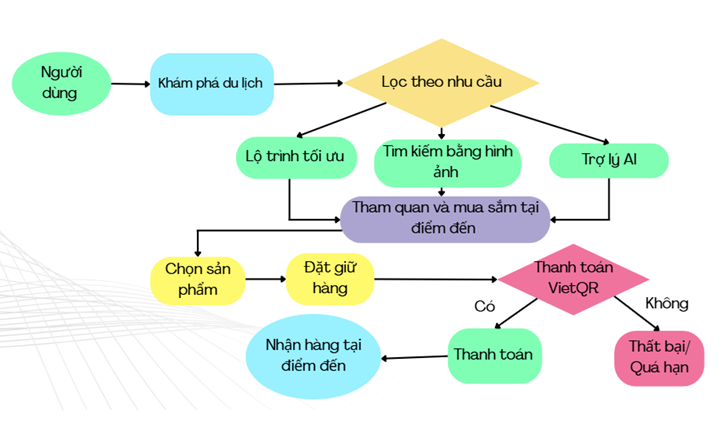
\includegraphics[width=0.9\textwidth]{images/Hinh1.png}
    \caption{Sơ đồ khái quát quy trình hệ thống AEGIS O2O}
    \label{fig:ct_mindmap}
\end{figure}
\subsection{Ánh xạ tư duy tính toán vào hệ thống}
Để tránh trình bày lý thuyết rời rạc, báo cáo chỉ giữ lại các quyết định có ảnh hưởng trực tiếp đến AEGIS O2O. Mỗi thành tố của Tư duy tính toán được gắn với một câu hỏi thiết kế, một giải pháp triển khai và một cách kiểm chứng cụ thể.

\begin{table}[H]
\centering
\renewcommand{\arraystretch}{1.35}
\small
\begin{adjustbox}{max width=\textwidth}
\begin{tabular}{|>{\raggedright\arraybackslash}p{2.9cm}|>{\raggedright\arraybackslash}p{3.7cm}|>{\raggedright\arraybackslash}p{4.5cm}|>{\raggedright\arraybackslash}p{4.0cm}|}
\hline
\textbf{Thành tố} & \textbf{Câu hỏi trong AEGIS} & \textbf{Quyết định thiết kế} & \textbf{Cách kiểm chứng} \\ \hline
Phân rã & Hệ thống nên tách bài toán lớn thành các phần nào? & Chia thành các nhóm việc: địa điểm, lộ trình, sản phẩm, giao dịch, trợ lý thông tin, dữ liệu mẫu và giao diện. & Kiểm tra từng ca sử dụng có phạm vi rõ ràng, không để một phần xử lý quá nhiều trách nhiệm. \\ \hline
Nhận diện mẫu & Những thao tác nào lặp lại trong nhiều chức năng? & Nhận ra các mẫu xử lý như tìm đối tượng gần vị trí người dùng, xếp hạng lựa chọn, giữ hàng tạm thời, xử lý ảnh và kiểm tra trạng thái tác vụ. & Đối chiếu từng chức năng với quy trình xử lý được trình bày ở chương cài đặt. \\ \hline
Trừu tượng hóa & Dữ liệu thực tế được biểu diễn ra sao để máy tính xử lý được? & Tọa độ được biểu diễn thành điểm địa lý; sản phẩm và cửa hàng thành bản ghi có thuộc tính; ảnh thành đặc trưng số; phiên giữ hàng thành trạng thái có thời hạn. & Kiểm tra lược đồ dữ liệu có ràng buộc rõ ràng, dữ liệu lỗi có cách xử lý và trạng thái nghiệp vụ không mơ hồ. \\ \hline
Thiết kế thuật toán & Quy trình nào cần chạy ngay, quy trình nào nên chạy nền? & Các bước nhẹ phản hồi trực tiếp cho người dùng; các bước nặng như xử lý ảnh, đồng bộ dữ liệu và dọn phiên hết hạn được chuyển sang tác vụ nền. & Kiểm thử chức năng, kiểm thử giao diện lập trình, kiểm thử đồng thời và đối chiếu kết quả trên dữ liệu thật. \\ \hline
\end{tabular}
\end{adjustbox}
\caption{Ánh xạ tư duy tính toán vào các quyết định thiết kế của AEGIS O2O}
\label{tab:ct_mapping}
\end{table}

Từ bảng trên, trọng tâm của báo cáo không phải là liệt kê càng nhiều công nghệ càng tốt, mà là chứng minh mỗi quyết định thiết kế đều gắn với một rủi ro cụ thể: tìm kiếm chậm, lộ trình thiếu hợp lý, bán vượt tồn kho, dữ liệu ảnh sản phẩm thiếu nhất quán, xử lý ảnh tốn thời gian hoặc câu trả lời thông minh thiếu dữ liệu kiểm chứng.

\clearpage
% ==============================================
% CHƯƠNG 2: CƠ SỞ LÝ THUYẾT VÀ CÔNG NGHỆ
% ==============================================
\section{Cơ sở công nghệ chọn lọc}

Mã nguồn của toàn bộ dự án AEGIS O2O được mở công khai tại mã lưu trữ: \url{https://github.com/just-mint/smart-tourism-system}.

Chương này chỉ trình bày những nền tảng trực tiếp được dùng trong kiến trúc AEGIS O2O. Các phần lý thuyết nền như TSP, tìm kiếm vector hoặc cơ chế khóa chỉ được giải thích ở mức đủ để hiểu quyết định thiết kế, tránh biến báo cáo thành phần tổng quan công nghệ quá rộng. Bạn có thể nhấn vào các nhóm bài toán trong bảng dưới đây để xem phần diễn giải chi tiết.

\begin{table}[H]
\centering
\renewcommand{\arraystretch}{1.35}
\small
\begin{adjustbox}{max width=\textwidth}
\begin{tabular}{|>{\raggedright\arraybackslash}p{3.1cm}|>{\raggedright\arraybackslash}p{4.0cm}|>{\raggedright\arraybackslash}p{4.6cm}|>{\raggedright\arraybackslash}p{3.7cm}|}
\hline
\textbf{Nhóm bài toán} & \textbf{Công nghệ/thuật toán} & \textbf{Vai trò trong hệ thống} & \textbf{Rủi ro cần kiểm soát} \\ \hline
\hyperref[sec:tech_spatial]{\textbf{Dữ liệu không gian}} & PostgreSQL/PostGIS\textsuperscript{[1]}, kiểu \texttt{geography}, GiST, \texttt{ST\_DWithin} & Tìm địa điểm/cửa hàng theo bán kính và sắp xếp theo khoảng cách. & Sai hệ tọa độ, truy vấn không dùng chỉ mục, bán kính quá lớn làm chậm API. \\ \hline
\hyperref[sec:tech_planner]{\textbf{Lập lịch trình}} & SAW/MCDM, OSRM\textsuperscript{[5]}, tham lam và 2-Opt & Xếp hạng điểm đến theo sở thích rồi sắp thứ tự di chuyển trong tập ứng viên nhỏ. & Thuật toán xấp xỉ không tối ưu tuyệt đối, OSRM quá thời gian chờ, trọng số tiêu chí thiếu hợp lệ. \\ \hline
\hyperref[sec:tech_inventory]{\textbf{Tồn kho O2O}} & Redis\textsuperscript{[8]} có thời hạn sống, PostgreSQL khóa mức dòng\textsuperscript{[2]}, mã đơn hàng duy nhất & Giữ hàng tạm thời, chống gửi lặp yêu cầu và giảm rủi ro bán vượt tồn. & Redis không phải nguồn sự thật cuối cùng; cần hoàn tác và dọn phiên giữ hết hạn trong PostgreSQL. \\ \hline
\hyperref[sec:tech_vision]{\textbf{Tìm kiếm bằng ảnh}} & \texttt{image\_url}, CLIP, pgvector\textsuperscript{[3]}, HNSW, khoảng cách cô-sin & Chuẩn hóa ảnh sản phẩm, mã hóa ảnh thành vector và tìm sản phẩm tương đồng trong kho. & Kết quả phụ thuộc chất lượng URL ảnh, độ phủ vector đặc trưng và tham số chỉ mục. \\ \hline
\hyperref[sec:tech_celery]{\textbf{Tác vụ nền}} & RabbitMQ, Celery\textsuperscript{[4]}, trạng thái tác vụ nền & Tách xử lý ảnh khỏi yêu cầu HTTP để giao diện không bị treo. & Tiến trình xử lý nền dừng giữa chừng, thông điệp bị xử lý lặp, tác vụ không cập nhật trạng thái. \\ \hline
Trợ lý ảo & Gọi công cụ với lược đồ tham số\textsuperscript{[7]} & Cho LLM gọi API nội bộ có kiểm soát thay vì tự tạo dữ liệu không có căn cứ. & Cần kiểm tra hợp lệ tham số, giới hạn quyền truy cập và ghi nhật ký công cụ đã gọi. \\ \hline
\end{tabular}
\end{adjustbox}
\caption{Các nền tảng kỹ thuật được giữ lại trong phạm vi báo cáo}
\label{tab:selected_technologies}
\end{table}

\subsection{Các nguyên tắc thiết kế rút ra}
\begin{enumerate}
    \item \textbf{Đưa phép tính về đúng tầng xử lý:} khoảng cách địa lý được tính trong PostGIS, tìm kiếm vector được thực hiện trong pgvector, còn máy chủ chỉ điều phối nghiệp vụ và kiểm tra quyền.
    \item \textbf{Không để AI quyết định trực tiếp dữ liệu nghiệp vụ:} LLM chỉ chọn công cụ và diễn giải kết quả; truy vấn thật vẫn do máy chủ kiểm soát bằng lược đồ tham số, phân quyền và giới hạn đầu vào.
    \item \textbf{Tách đường xử lý nhanh và xử lý chậm:} API phản hồi ngay khi tác vụ AI được ghi nhận, phần mã hóa ảnh và truy vấn tương đồng được chuyển sang tiến trình nền; riêng dữ liệu ảnh sản phẩm được chuẩn hóa bằng tập lệnh xử lý hàng loạt trước khi đồng bộ vector.
    \item \textbf{Cơ sở dữ liệu là lớp bảo vệ cuối cùng:} Redis hỗ trợ thời hạn sống và bộ nhớ đệm cho trải nghiệm giữ hàng, nhưng tính đúng của tồn kho phải dựa vào giao dịch PostgreSQL, ràng buộc dữ liệu và khóa mức dòng.
\end{enumerate}

\subsection{Nền tảng dữ liệu không gian và truy vấn theo bán kính}
\label{sec:tech_spatial}
Dữ liệu du lịch và thương mại địa phương luôn gắn với vị trí vật lý. Nếu chỉ lưu vĩ độ, kinh độ dưới dạng hai số thực và tự tính khoảng cách ở máy chủ, hệ thống dễ gặp ba vấn đề: sai công thức khi đổi hệ tọa độ, không tận dụng được chỉ mục không gian và khó lọc hiệu quả khi dữ liệu tăng. Vì vậy AEGIS O2O dùng PostgreSQL kết hợp PostGIS\textsuperscript{[1]} để biểu diễn tọa độ bằng kiểu dữ liệu không gian và thực hiện các phép lọc trực tiếp tại cơ sở dữ liệu.

Trong các truy vấn như tìm địa điểm hoặc cửa hàng quanh vị trí hiện tại, hệ thống dùng tư duy lọc hai bước. Bước thứ nhất là giới hạn tập ứng viên bằng bán kính với \texttt{ST\_DWithin}; bước thứ hai là sắp xếp lại theo khoảng cách thực tế bằng \texttt{ST\_Distance}. Cách này phù hợp với bản chất của bài toán: người dùng không cần toàn bộ dữ liệu, mà chỉ cần một tập nhỏ đủ gần để tiếp tục xem chi tiết, lập lịch trình hoặc mua sắm. Về mặt thiết kế, tham số bán kính cần được giới hạn ở API để tránh việc một yêu cầu vô tình biến thành truy vấn quét toàn bộ dữ liệu.

\subsection{Cơ sở lập lịch trình thông minh}
\label{sec:tech_planner}
Bài toán lập lịch trình trong AEGIS không chỉ là tìm đường ngắn nhất. Một điểm dừng tốt còn phụ thuộc vào danh mục, độ phù hợp với sở thích, ngân sách, thời gian di chuyển và mức độ ưu tiên của người dùng. Vì vậy hệ thống tách bài toán thành hai tầng: tầng xếp hạng ứng viên và tầng sắp thứ tự di chuyển.

Ở tầng xếp hạng, hệ thống dùng phương pháp ra quyết định đa tiêu chí, cụ thể là chuẩn hóa các tiêu chí rồi cộng trọng số theo mô hình SAW. Cách làm này giúp biến những yếu tố khác loại như khoảng cách, chi phí, độ ưu tiên danh mục và điểm đánh giá thành một điểm số so sánh được. Ở tầng lộ trình, sau khi đã giới hạn còn một số điểm dừng nhỏ, hệ thống dùng cách chọn điểm gần nhất để tạo tuyến ban đầu, sau đó dùng 2-Opt để cải thiện bằng cách hoán đổi hai cạnh và loại bỏ các đoạn giao nhau không cần thiết. Đây là lựa chọn thực dụng cho bài toán TSP: không tìm nghiệm tối ưu tuyệt đối cho mọi trường hợp, nhưng trả về tuyến hợp lý đủ nhanh trong phiên tương tác của người dùng.

\subsection{Kiểm soát tồn kho O2O trong môi trường đồng thời}
\label{sec:tech_inventory}
Trong thương mại O2O, rủi ro nghiêm trọng nhất là bán vượt tồn kho khi nhiều người dùng cùng đặt giữ một sản phẩm. AEGIS xử lý vấn đề này bằng cách xem PostgreSQL là nguồn dữ liệu quyết định cuối cùng. Khi giữ hàng, máy chủ mở giao dịch, khóa dòng tồn kho liên quan bằng cơ chế khóa mức dòng\textsuperscript{[2]}, kiểm tra lượng hàng khả dụng, cập nhật \texttt{locked\_stock} và tạo bản ghi \texttt{InventoryLock} có thời hạn.

Redis\textsuperscript{[8]} chỉ được dùng để hỗ trợ thời hạn sống, bộ nhớ đệm và hiển thị trải nghiệm thời gian giữ hàng. Điều này quan trọng vì Redis có thể nhanh nhưng không nên là nơi quyết định tính đúng của giao dịch. Nếu Redis gặp lỗi hoặc khóa tạm hết hạn không đúng thời điểm, PostgreSQL vẫn còn bản ghi giữ hàng và trạng thái tồn kho để bộ lập lịch Celery hoặc tác vụ dọn dẹp xử lý. Cách phân vai này giúp hệ thống giảm rủi ro lỗi tương tranh, đồng thời vẫn giữ được trải nghiệm phản hồi nhanh trên giao diện.

\subsection{Tìm kiếm vector và mô hình CLIP}
\label{sec:tech_vision}
Tìm kiếm bằng ảnh là bài toán khó vì ảnh tải lên của người dùng không thể so khớp bằng tên sản phẩm đơn thuần. Hệ thống cần chuyển ảnh thành một biểu diễn số học có khả năng phản ánh đặc trưng thị giác. AEGIS dùng CLIP để mã hóa ảnh thành vector đặc trưng, sau đó lưu vào cột \texttt{embedding} của sản phẩm và truy vấn độ tương đồng bằng pgvector\textsuperscript{[3]}.

Về mặt chỉ mục, tìm kiếm vector trên tập dữ liệu lớn không nên dùng quét tuyến tính vì chi phí tăng theo số sản phẩm và số chiều vector. HNSW được dùng như một chỉ mục tìm kiếm láng giềng gần đúng để giảm độ trễ, chấp nhận đánh đổi một phần rất nhỏ về độ chính xác tuyệt đối. Vì vậy khi đánh giá phân hệ tìm kiếm bằng ảnh, không thể chỉ đo thời gian phản hồi; cần đo thêm độ phủ sản phẩm có vector đặc trưng, tỉ lệ ảnh lỗi, tỉ lệ tìm đúng trong nhóm kết quả đầu và chất lượng kết quả theo từng nhóm sản phẩm.

\subsection{Tác vụ nền và xử lý bất đồng bộ}
\label{sec:tech_celery}
Một số thao tác trong hệ thống có thời gian xử lý không ổn định, đặc biệt là tải ảnh, chạy mô hình CLIP, đồng bộ vector đặc trưng và dọn phiên giữ hàng hết hạn. Nếu ép các thao tác này chạy đồng bộ trong yêu cầu HTTP, người dùng sẽ phải chờ lâu và API dễ quá thời gian chờ. Vì vậy AEGIS dùng RabbitMQ và Celery\textsuperscript{[4]} để chuyển các công việc chậm sang tiến trình nền.

Mô hình bất đồng bộ được thiết kế theo hướng lưu trạng thái trước, xử lý sau. API nhận yêu cầu, ghi một bản ghi tác vụ với trạng thái ban đầu, trả \texttt{task\_id} cho giao diện, sau đó tiến trình nền cập nhật kết quả vào cơ sở dữ liệu. Giao diện không chờ kết nối HTTP dài, mà hỏi trạng thái định kỳ qua API để lấy kết quả khi tác vụ hoàn tất. Thiết kế này làm rõ ranh giới trách nhiệm: API chịu trách nhiệm nhận và xác thực yêu cầu; tiến trình nền chịu trách nhiệm xử lý nặng; cơ sở dữ liệu lưu trạng thái trung gian để hệ thống có thể phục hồi khi tiến trình nền lỗi.

\subsection{Kiến trúc ứng dụng web trang đơn và giao tiếp REST}
Phía trình duyệt của AEGIS được xây dựng theo mô hình SPA. Nginx hoặc Vite chỉ phục vụ tài nguyên tĩnh như HTML, JavaScript và CSS; sau khi tải xong, chính trình duyệt của người dùng thực thi React và gọi API đến FastAPI\textsuperscript{[6]}. Vì vậy khi thiết kế kiến trúc, cần phân biệt rõ hai luồng: luồng tải ứng dụng từ máy chủ web và luồng API do trình duyệt gửi đến máy chủ nghiệp vụ. Cách hiểu này giúp tránh vẽ sai sơ đồ mạng, đồng thời làm rõ nơi xử lý mã phiên, lỗi 401/403, trạng thái đang tải và thử lại yêu cầu.

REST API được dùng cho các nghiệp vụ có cấu trúc rõ như đăng nhập, truy vấn địa điểm, lập lịch trình, lấy danh mục sản phẩm và tạo đơn. Với các tác vụ bất đồng bộ, API không trả kết quả cuối ngay lập tức mà trả một mã tác vụ; giao diện hỏi trạng thái định kỳ. Cách thiết kế này giữ cho giao diện phản hồi nhanh hơn, giảm nguy cơ quá thời gian chờ và giúp máy chủ có thể mở rộng tiến trình nền độc lập với số lượng tiến trình web.

\subsection{Bảo mật ứng dụng và phân quyền}
Hệ thống có nhiều nhóm người dùng khác nhau: du khách, người bán và quản trị viên. Vì vậy cơ sở lý thuyết về bảo mật không chỉ nằm ở đăng nhập, mà còn ở phân quyền theo tài nguyên. Người dùng thường chỉ được xem hoặc tạo giao dịch của chính mình; người bán chỉ nên quản lý cửa hàng thuộc quyền sở hữu; quản trị viên có quyền cao hơn nhưng vẫn cần được ghi nhận thao tác nhạy cảm.

Ở tầng xác thực, mật khẩu phải được băm một chiều và mã phiên làm việc phải có thời hạn. Ở tầng API, các điểm truy cập thay đổi trạng thái như tạo phiên giữ hàng, tạo đơn, xác nhận thanh toán hoặc cập nhật sản phẩm cần kiểm tra quyền trước khi ghi dữ liệu. Ở tầng dữ liệu, các ràng buộc như giá không âm, tồn kho không âm, lượng hàng đang giữ không âm và mã đơn hàng duy nhất giúp giảm rủi ro lỗi ứng dụng làm hỏng dữ liệu nghiệp vụ.

\subsection{Đóng gói, cấu hình môi trường và tái lập kết quả}
AEGIS sử dụng Docker Compose để gom các thành phần phụ thuộc như PostgreSQL, Redis, RabbitMQ, máy chủ nghiệp vụ và giao diện vào một môi trường có thể tái lập. Đồng thời, cấu hình kết nối cơ sở dữ liệu được tách qua biến môi trường để cùng một mã nguồn có thể chạy với PostgreSQL cục bộ, cơ sở dữ liệu trong môi trường đóng gói hoặc môi trường triển khai thật. Cách tổ chức này giúp kết quả kiểm thử có nguồn dữ liệu rõ ràng và dễ tái hiện giữa các máy phát triển.

Nguyên tắc triển khai là tách cấu hình khỏi mã nguồn bằng biến môi trường. Các giá trị như \texttt{POSTGRES\_SERVER}, \texttt{POSTGRES\_PORT}, \texttt{REDIS\_URL}, \texttt{RABBITMQ\_URL}, \texttt{VITE\_API\_URL} và khóa bí mật thanh toán phải được cấu hình theo từng môi trường. Việc này giúp cùng một mã nguồn có thể chạy ở ba chế độ: phát triển cục bộ, demo bằng Docker và triển khai lên máy chủ đám mây.

\clearpage
% ==============================================
% CHƯƠNG 3: PHÂN TÍCH VÀ THIẾT KẾ HỆ THỐNG
% ==============================================
\section{Phân tích và thiết kế hệ thống}
\subsection{Phân tích yêu cầu hệ thống}
Mục tiêu cốt lõi của dự án AEGIS là hỗ trợ chu trình trải nghiệm của du khách từ khám phá địa điểm, lập lịch trình, tìm sản phẩm địa phương đến đặt giữ hàng tại cửa hàng. Hệ thống được phân tích theo ba nhóm tác nhân chính:

\begin{itemize}
    \item \textbf{Du khách:} tìm kiếm địa điểm, xem câu chuyện văn hóa, tạo lịch trình, xem sản phẩm có ảnh minh họa, tìm sản phẩm bằng ảnh, đặt giữ hàng và nhận mã xác thực.
    \item \textbf{Cơ sở kinh doanh:} quản lý sản phẩm, tồn kho, xác nhận mã nhận hàng và cập nhật trạng thái đơn.
    \item \textbf{Quản trị hệ thống:} quản lý dữ liệu nền, kiểm tra tác vụ nền, theo dõi lỗi và xử lý các giao dịch bất thường.
\end{itemize}

Các ca sử dụng trọng tâm được đặc tả như sau:

\begin{table}[H]
\centering
\renewcommand{\arraystretch}{1.35}
\small
\begin{adjustbox}{max width=\textwidth}
\begin{tabular}{|>{\raggedright\arraybackslash}p{3.0cm}|>{\raggedright\arraybackslash}p{3.2cm}|>{\raggedright\arraybackslash}p{4.2cm}|>{\raggedright\arraybackslash}p{4.2cm}|}
\hline
\textbf{Ca sử dụng} & \textbf{Tác nhân chính} & \textbf{Luồng chính} & \textbf{Luồng lỗi cần xử lý} \\ \hline
Khám phá địa điểm & Du khách & Nhập từ khóa hoặc dùng vị trí hiện tại; hệ thống truy vấn địa điểm/cửa hàng trong bán kính và hiển thị trên bản đồ. & Thiếu quyền vị trí, dữ liệu tọa độ không hợp lệ, không có kết quả trong bán kính. \\ \hline
Lập lịch trình & Du khách & Chọn sở thích, ngân sách, số điểm dừng; hệ thống xếp hạng ứng viên, lấy ma trận OSRM, chạy thuật toán tham lam và 2-Opt rồi trả về tuyến đường. & OSRM quá thời gian chờ, số điểm dừng quá ít, trọng số tiêu chí không hợp lệ. \\ \hline
Tìm kiếm bằng ảnh & Du khách & Tải ảnh lên; API lưu tập tin hợp lệ, tạo \texttt{VisionTask} trạng thái \texttt{processing}; tiến trình nền trích xuất vector đặc trưng và trả về sản phẩm tương đồng. & Tập tin quá lớn, sai kiểu MIME, ảnh hỏng, tiến trình nền lỗi, không có vector sản phẩm. \\ \hline
Đặt giữ sản phẩm O2O & Du khách, Cơ sở kinh doanh & Du khách đặt giữ hàng; hệ thống khóa tồn kho tạm thời, tạo mã xác thực; cửa hàng kiểm tra mã khi khách đến nhận. & Hết hàng, phiên giữ hết hạn, gửi lặp yêu cầu, nhân viên xác nhận sai mã. \\ \hline
\end{tabular}
\end{adjustbox}
\caption{Các ca sử dụng trọng tâm và luồng lỗi cần kiểm soát}
\label{tab:use_cases}
\end{table}

Bên cạnh yêu cầu chức năng, hệ thống cần đáp ứng một số yêu cầu phi chức năng: phản hồi API thông thường trong ngưỡng vài trăm mili-giây trên dữ liệu mẫu; tác vụ AI không làm nghẽn máy chủ web; giao dịch tồn kho phải kiểm soát được thao tác gửi lặp; tập tin ảnh đầu vào cần giới hạn kích thước và kiểu MIME; dữ liệu sản phẩm mẫu cần có \texttt{image\_url} đủ ổn định để hiển thị và sinh vector đặc trưng; các API nhạy cảm cần xác thực người dùng và phân quyền theo vai trò.

\subsection{Thiết kế kiến trúc tổng thể}

Hệ thống được thiết kế dựa trên phương pháp luận \textbf{Thiết kế hướng miền nghiệp vụ} kết hợp kiến trúc dịch vụ tách theo chức năng. Trong phạm vi đồ án, các miền nghiệp vụ được triển khai chung trong máy chủ FastAPI nhưng vẫn giữ ranh giới mô-đun, lược đồ dữ liệu và API rõ ràng; khi cần mở rộng, những phần xử lý nặng như lập lịch trình hoặc xử lý ảnh có thể tách thành dịch vụ độc lập. Các nghiệp vụ cốt lõi được phân hoạch như sau:

\begin{itemize}
    \item \textbf{Phân hệ không gian:} Chịu trách nhiệm quản lý cấu trúc dữ liệu vị trí, tọa độ địa lý và thực thi các phép toán phân tích không gian.
    
    \item \textbf{Phân hệ tồn kho và giao dịch:} Quản lý thông tin cơ sở kinh doanh, danh mục sản phẩm, đồng thời đảm bảo tính toàn vẹn của các phiên giao dịch thông qua cơ chế kiểm soát đồng bộ hóa tài nguyên nguyên tử.
    
    \item \textbf{Phân hệ thị giác máy tính:} Tiếp nhận dữ liệu hình ảnh đầu vào và điều phối các tác vụ trích xuất đặc trưng của mô hình học sâu thông qua hệ thống hàng đợi xử lý bất đồng bộ.

    \item \textbf{Phân hệ dữ liệu sản phẩm:} Chuẩn hóa dữ liệu mẫu cho sản phẩm O2O, đặc biệt là \texttt{name}, \texttt{description} và \texttt{image\_url}, để giao diện hiển thị nhất quán và quy trình đồng bộ vector có nguồn ảnh đầu vào.
    
    \item \textbf{Phân hệ lập kế hoạch:} Chịu trách nhiệm thiết lập lịch trình tham quan, điều phối các luồng giao tiếp nội bộ tới dịch vụ tối ưu hóa thuật toán.
    
    \item \textbf{Phân hệ trợ lý ảo:} Quản lý trợ lý AI, tích hợp khả năng xử lý ngôn ngữ tự nhiên để phân tích ý định người dùng và chuyển thành lệnh gọi các chức năng hệ thống đã được kiểm soát.
\end{itemize}

Kiến trúc tổng thể của hệ thống được minh họa chi tiết tại \hyperref[fig:aegis_architecture]{[Hình \ref*{fig:aegis_architecture}]}.

\begin{figure}[H]
  \centering
  \resizebox{\textwidth}{!}{%
  \begin{tikzpicture}[
    clientbox/.style={draw=blue!80, thick, rounded corners, fill=blue!10, align=center, font=\small, minimum width=4.1cm, minimum height=1.05cm},
    gatewaybox/.style={draw=orange!80, thick, rounded corners, fill=orange!10, align=center, font=\small, minimum width=4.1cm, minimum height=1.05cm},
    corebox/.style={draw=green!80!black, thick, rounded corners, fill=green!10, align=center, font=\small, minimum width=4.1cm, minimum height=1.05cm},
    servicebox/.style={draw=purple!80, thick, rounded corners, fill=purple!10, align=center, font=\small, minimum width=3.8cm, minimum height=1.0cm},
    dbbox/.style={draw=teal!80, thick, rounded corners, fill=teal!10, align=center, font=\small, minimum width=3.8cm, minimum height=1.0cm},
    label/.style={font=\small, fill=white, inner sep=1pt},
    every path/.style={thick, color=gray!80!black}
  ]
    \node[clientbox] (browser) at (0,5.0) {Trình duyệt người dùng\\chạy giao diện React};
    \node[gatewaybox] (gateway) at (0,3.3) {Cổng Traefik\\mã hóa và chuyển tiếp};
    \node[corebox] (nginx) at (-4.7,1.5) {Nginx\\trả tài nguyên giao diện};
    \node[corebox] (api) at (4.7,1.5) {Máy chủ FastAPI\\API nghiệp vụ};
    
    \node[servicebox] (opt) at (-2.7,-0.5) {Dịch vụ tối ưu\\MCDM + TSP};
    \node[servicebox] (rabbit) at (2.7,-0.5) {RabbitMQ\\hàng đợi tác vụ};
    \node[servicebox] (worker) at (2.7,-2.5) {Celery\\xử lý ảnh và dọn phiên giữ};
    \node[dbbox] (redis) at (7.4,-0.5) {Redis\\thời hạn sống và bộ nhớ đệm};
    \node[dbbox] (db) at (7.4,-2.5) {PostgreSQL\\PostGIS + pgvector};

    \draw[->] (browser) -- node[label, right]{Truy cập HTTPS} (gateway);
    \draw[->] (gateway) -- node[label, above left]{Tải giao diện} (nginx);
    \draw[->] (nginx) -- node[label, left]{Tài nguyên tĩnh} (browser);
    \draw[->, very thick] (gateway) -- node[label, above right]{Luồng API} (api);
    \draw[->] (api) -- (opt);
    \draw[->] (api) -- (rabbit);
    \draw[->] (rabbit) -- (worker);
    \draw[->] (api) -- (redis);
    \draw[->] (api) -- (db);
    \draw[->] (worker) -- (db);
  \end{tikzpicture}%
  }
  \vspace{0.3cm}
  \caption{Sơ đồ kiến trúc dịch vụ AEGIS O2O: trình duyệt gọi API qua Traefik đến FastAPI; Nginx chỉ phục vụ tài nguyên tĩnh của giao diện React}
  \label{fig:aegis_architecture}
\end{figure}

\subsection{Thiết kế cơ sở dữ liệu}
Hình và bảng dưới đây trình bày sơ đồ thực thể liên kết của hệ thống. Nội dung này cung cấp cái nhìn tổng quan về cấu trúc các bảng dữ liệu lõi và mối quan hệ giữa các miền nghiệp vụ. Cơ sở dữ liệu PostgreSQL được thiết kế theo hướng chuẩn hóa các thực thể chính và tích hợp dữ liệu không gian, thương mại O2O và AI. Để tránh sai lệch giữa báo cáo và mã nguồn, bảng dưới đây được đối chiếu trực tiếp với các mô hình hiện tại trong \texttt{backend/app/\allowbreak domains/\allowbreak inventory/\allowbreak model.py}, \texttt{backend/app/\allowbreak domains/\allowbreak culture/\allowbreak model.py}, \texttt{backend/app/\allowbreak domains/\allowbreak vision/\allowbreak model.py} và \texttt{backend/app/\allowbreak models.py}.

\begin{table}[H]
\centering
\renewcommand{\arraystretch}{1.2}
\scriptsize
\begin{adjustbox}{max width=\textwidth}
\begin{tabular}{|>{\raggedright\arraybackslash}p{3.0cm}|>{\raggedright\arraybackslash}p{9.3cm}|>{\raggedright\arraybackslash}p{3.2cm}|}
\hline
\textbf{Bảng} & \textbf{Cột chính trong mã nguồn hiện tại} & \textbf{Vai trò nghiệp vụ} \\ \hline
\texttt{user} & \texttt{id}, \texttt{email}, \texttt{hashed\_password}, \texttt{full\_name}, \texttt{is\_active}, \texttt{is\_superuser}, \texttt{created\_at} & Xác thực, phân quyền cơ bản \\ \hline
\texttt{places} & \texttt{id}, \texttt{place\_id}, \texttt{place\_type}, \texttt{name}, \texttt{category}, \texttt{address}, \texttt{lat}, \texttt{lon}, \texttt{geom}, \texttt{phone}, \texttt{rating}, \texttt{review\_count}, \texttt{image\_url} & Địa điểm du lịch/văn hóa \\ \hline
\texttt{reviews} & \texttt{id}, \texttt{place\_id}, \texttt{author\_name}, \texttt{rating}, \texttt{text}, \texttt{time\_posted} & Đánh giá địa điểm \\ \hline
\texttt{stores} & \texttt{store\_id}, \texttt{place\_id}, \texttt{name}, \texttt{category}, \texttt{address}, \texttt{lat}, \texttt{lon}, \texttt{geom}, \texttt{phone}, \texttt{rating} & Cửa hàng O2O gắn với vị trí \\ \hline
\texttt{products} & \texttt{product\_id}, \texttt{name}, \texttt{description}, \texttt{price}, \texttt{original\_price}, \texttt{image\_url}, \texttt{embedding}, \texttt{embedding\_model}, \texttt{embedding\_version}, \texttt{embedded\_at}, \texttt{size}, \texttt{color}, \texttt{tags}, \texttt{created\_at} & Danh mục sản phẩm và dữ liệu vector \\ \hline
\texttt{inventory} & \texttt{inventory\_id}, \texttt{store\_id}, \texttt{product\_id}, \texttt{stock}, \texttt{version}, \texttt{locked\_stock}, \texttt{price\_override} & Tồn kho theo từng cửa hàng \\ \hline
\texttt{inventory\_locks} & \texttt{id}, \texttt{product\_id}, \texttt{store\_id}, \texttt{user\_id}, \texttt{quantity}, \texttt{locked\_at}, \texttt{expires\_at}, \texttt{status} & Khóa giữ hàng tạm thời \\ \hline
\texttt{orders} & \texttt{order\_id}, \texttt{user\_id}, \texttt{product\_id}, \texttt{store\_id}, \texttt{lock\_id}, \texttt{quantity}, \texttt{total\_amount}, \texttt{full\_name}, \texttt{phone}, \texttt{address}, \texttt{status}, \texttt{order\_code}, \texttt{created\_at} & Đơn hàng O2O \\ \hline
\texttt{payments} & \texttt{payment\_id}, \texttt{order\_id}, \texttt{provider}, \texttt{amount}, \texttt{currency}, \texttt{status}, \texttt{transaction\_id}, \texttt{idempotency\_key}, \texttt{raw\_payload}, \texttt{created\_at}, \texttt{updated\_at} & Ghi nhận thanh toán/VietQR mô phỏng \\ \hline
\texttt{vision\_tasks} & \texttt{id}, \texttt{task\_id}, \texttt{image\_path}, \texttt{status}, \texttt{detected\_objects}, \texttt{matched\_product\_ids}, \texttt{created\_at} & Trạng thái scan ảnh bất đồng bộ \\ \hline
\texttt{virtual\_closets} & \texttt{id}, \texttt{user\_id}, \texttt{image\_path}, \texttt{vector\_embedding}, \texttt{embedding\_model}, \texttt{embedding\_version}, \texttt{embedded\_at}, \texttt{created\_at} & Tủ đồ ảo và phối đồ \\ \hline
\texttt{inventory\_events} & \texttt{id}, \texttt{entity\_type}, \texttt{entity\_id}, \texttt{user\_id}, \texttt{action}, \texttt{payload}, \texttt{created\_at} & Nhật ký kiểm toán cho tồn kho/đơn hàng \\ \hline
\end{tabular}
\end{adjustbox}
\caption{Lược đồ dữ liệu cốt lõi đối chiếu với mã nguồn hiện tại}
\label{tab:code_aligned_schema}
\end{table}

Phiên bản hiện tại tập trung mô tả các bảng và cột đã có trong mã nguồn. Các mở rộng cho bản thương mại như \texttt{opening\_hours}, \texttt{service\_radius}, \texttt{product\_categories}, \texttt{embedding\_status} hoặc \texttt{is\_merchant} được tách sang phần hướng phát triển để giữ lược đồ trong báo cáo khớp với hệ thống đang chạy.

Các ràng buộc dữ liệu quan trọng ở mức cơ sở dữ liệu bao gồm: giá sản phẩm không âm, \texttt{stock >= 0}, \texttt{locked\_stock >= 0}, \texttt{locked\_stock <= stock}, số tiền thanh toán không âm và mã đơn hàng \texttt{order\_code} là duy nhất. Những ràng buộc này giúp giảm sự phụ thuộc vào việc kiểm tra ở tầng ứng dụng, biến cơ sở dữ liệu thành lớp phòng thủ cuối cùng chống lại lỗi tương tranh khi có nhiều luồng đặt hàng cùng lúc.

\subsection{Mô hình luồng dữ liệu nghiệp vụ cốt lõi}
Phân tích quy trình di chuyển dữ liệu của chức năng \textbf{chuẩn hóa dữ liệu sản phẩm, tìm kiếm bằng ảnh và tạo giao dịch O2O}:
\begin{enumerate}
    \item \textbf{[Tập lệnh dữ liệu $\rightarrow$ CSDL]:} \texttt{fix\_product\_\allowbreak images.py} đọc \texttt{products}, \texttt{inventory} và \texttt{stores}; dựa vào \texttt{stores.category} để chọn nhóm ảnh đồ uống/ẩm thực, thời trang, quà lưu niệm hoặc nhóm mặc định; sau đó cập nhật \texttt{name}, \texttt{description} và \texttt{image\_url} cho mỗi \texttt{product\_id} một lần.
    \item \textbf{[Đồng bộ vector $\rightarrow$ CSDL]:} \texttt{sync\_product\_\allowbreak vectors.py} tải ảnh từ \texttt{image\_url}, chạy CLIP-ViT-B-32 và lưu vector 512 chiều vào \texttt{products.embedding}. Sản phẩm thiếu URL hoặc tải ảnh lỗi sẽ bị bỏ qua hoặc ghi nhận lỗi để xử lý sau.
    \item \textbf{[Trình duyệt $\rightarrow$ API]:} Trình duyệt gửi tập tin ảnh lên điểm truy cập \texttt{/api/v1/\allowbreak vision/\allowbreak scan}. API kiểm tra kiểu MIME, dung lượng, nội dung ảnh và lưu tập tin bằng tên UUID để tránh ghi đè.
    \item \textbf{[API $\rightarrow$ RabbitMQ]:} FastAPI ghi bản ghi \texttt{VisionTask} với trạng thái \texttt{processing}, đưa tác vụ \texttt{workers.\allowbreak ai\_worker.\allowbreak vision\_tasks.\allowbreak process\_image} vào Celery và trả về \texttt{task\_id}. Điểm truy cập hiện trả \texttt{HTTP 202 Accepted} theo đúng chuẩn API tác vụ nền.
    \item \textbf{[Trình duyệt $\rightarrow$ API]:} Trình duyệt gọi \texttt{/api/v1/\allowbreak vision/\allowbreak tasks/\allowbreak \{task\_id\}} để kiểm tra trạng thái; nếu tác vụ xử lý quá lâu, API chuyển trạng thái sang \texttt{failed}.
    \item \textbf{[RabbitMQ $\rightarrow$ Tiến trình nền]:} Tiến trình Celery đọc ảnh, chạy mô hình CLIP trích xuất vector 512 chiều và truy vấn pgvector theo khoảng cách cô-sin.
    \item \textbf{[Tiến trình nền $\rightarrow$ CSDL]:} Tiến trình nền lấy tối đa 4 sản phẩm tương đồng, bổ sung thông tin cửa hàng còn hàng, cập nhật \texttt{matched\_product\_ids}, \texttt{detected\_objects} và chuyển trạng thái tác vụ sang \texttt{completed}.
    \item \textbf{[Trình duyệt $\rightarrow$ CSDL/Redis]:} Người dùng chọn sản phẩm và bấm nút mua. Hệ thống khóa dòng \texttt{inventory} trong PostgreSQL, tạo bản ghi giữ hàng rồi ghi thời hạn sống vào Redis để hỗ trợ trạng thái giữ tồn kho tạm thời và mở hộp thanh toán VietQR.
\end{enumerate}
Tiến trình nền không trả kết quả trực tiếp về tiến trình FastAPI đang xử lý yêu cầu tải ảnh. Kết quả được ghi xuống PostgreSQL, sau đó trình duyệt lấy lại qua vòng hỏi trạng thái định kỳ ở điểm truy cập \texttt{/api/v1/vision/tasks/\{task\_id\}}. Các trạng thái thất bại được ghi nhận rõ trong luồng này: nếu ảnh không hợp lệ, API từ chối bằng mã lỗi 413/415; nếu tác vụ không được đưa vào hàng đợi hoặc xử lý quá lâu, trạng thái chuyển sang \texttt{failed}; nếu không tìm thấy sản phẩm tương đồng, giao diện hiển thị trạng thái rỗng thay vì tạo đơn; nếu giữ tồn kho thất bại, API trả lỗi nghiệp vụ để người dùng chọn cửa hàng khác.

\begin{table}[H]
\centering
\renewcommand{\arraystretch}{1.25}
\small
\begin{adjustbox}{max width=\textwidth}
\begin{tabular}{|>{\raggedright\arraybackslash}p{2.4cm}|>{\raggedright\arraybackslash}p{5.5cm}|>{\raggedright\arraybackslash}p{6.8cm}|}
\hline
\textbf{Luồng} & \textbf{Điểm truy cập/tác vụ} & \textbf{Kết quả chính} \\ \hline
Tải ảnh tìm kiếm & \texttt{POST /api/v1/\allowbreak vision/\allowbreak scan} & Lưu tập tin, tạo \texttt{VisionTask(status="processing")}, đưa tác vụ vào Celery, trả \texttt{task\_id}. \\ \hline
Hỏi trạng thái ảnh & \texttt{GET /api/v1/\allowbreak vision/\allowbreak tasks/\allowbreak \{task\_id\}} & Đọc kết quả từ cơ sở dữ liệu; trả \texttt{processing}, \texttt{completed} hoặc \texttt{failed}. \\ \hline
Xử lý ảnh nền & \texttt{process\_image(...)} & Mã hóa ảnh bằng CLIP, truy vấn khoảng cách cô-sin trên \texttt{Product.embedding}, lấy tối đa 4 kết quả và cập nhật tác vụ. \\ \hline
Tạo giao dịch O2O & \texttt{POST /api/v1/\allowbreak inventory/\allowbreak lock} và \texttt{POST /api/v1/\allowbreak inventory/\allowbreak orders} & Khóa tồn kho theo \texttt{store\_id/\allowbreak product\_id}, tạo \texttt{Order} và \texttt{Payment(pending)}. \\ \hline
\end{tabular}
\end{adjustbox}
\caption{Luồng tìm kiếm bằng ảnh và tạo giao dịch O2O đối chiếu với điểm truy cập trong mã nguồn}
\label{tab:vision_o2o_flow}
\end{table}

Bên cạnh tìm kiếm bằng ảnh, lập lịch trình thông minh là luồng dữ liệu lớn thứ hai của hệ thống. Đây là quy trình giúp người dùng nhanh chóng tạo ra một lịch trình di chuyển hợp lý dựa trên sở thích cá nhân. Người dùng nhập vị trí hiện tại, bán kính, từ khóa, ngân sách, số điểm dừng và trọng số ưu tiên; máy chủ tự lọc ứng viên phù hợp rồi trả về lộ trình đã sắp thứ tự cho giao diện hiển thị.

\begin{enumerate}
    \item \textbf{[Trình duyệt $\rightarrow$ API lập lịch trình]:} Giao diện gọi \texttt{POST /api/v1/planner/generate} với tọa độ hiện tại, bán kính, từ khóa, ngân sách và trọng số \texttt{rating/distance/price}.
    \item \textbf{[API lập lịch trình $\rightarrow$ PostGIS]:} Máy chủ lọc cửa hàng trong bán kính bằng \texttt{ST\_DWithin}, loại cửa hàng không có tồn kho khả dụng và loại ứng viên vượt ngân sách.
    \item \textbf{[API lập lịch trình $\rightarrow$ Dịch vụ tối ưu]:} Máy chủ gửi danh sách ứng viên sang \texttt{POST /api/v1/optimize}; dịch vụ áp dụng phân tích ngữ cảnh, xếp hạng MCDM, chọn \texttt{top\_n} và chạy quy trình TSP.
    \item \textbf{[Dịch vụ tối ưu $\rightarrow$ OSRM]:} Dịch vụ ưu tiên OSRM Table/Route để lấy ma trận thời gian và hình dạng đường đi; nếu OSRM lỗi thì chuyển sang Haversine để vẫn trả được lộ trình.
    \item \textbf{[API lập lịch trình $\rightarrow$ CSDL $\rightarrow$ Trình duyệt]:} Máy chủ gắn tối đa 5 sản phẩm nổi bật cho mỗi cửa hàng trong tuyến, đóng gói \texttt{optimized\_route}, \texttt{metrics}, \texttt{route\_geometry} và trả về giao diện.
\end{enumerate}

\clearpage
% ==============================================
% CHƯƠNG 4: CHI TIẾT CÀI ĐẶT
% ==============================================
\section{Chi tiết cài đặt các phân hệ và thuật toán}
Chương này bóc tách mã nguồn thực tế để minh họa việc chuyển đổi từ tư duy thiết kế thành sản phẩm phần mềm.

\subsection{Phân hệ không gian}
Đoạn mã giải quyết bài toán tìm kiếm theo bán kính. Thuật toán đẩy gánh nặng tính toán xuống tầng cơ sở dữ liệu bằng hàm \texttt{ST\_DWithin} và kiểu \texttt{Geography} để tính khoảng cách phù hợp hơn trên bề mặt Trái Đất so với mô hình phẳng đơn giản. Việc này tận dụng tốt chỉ mục GiST của PostGIS\textsuperscript{[1]}.

\begin{lstlisting}[language=SQL, caption={Truy vấn không gian theo bán kính}]
SELECT id, name, address,
       ST_Distance(
           geom::geography,
           ST_SetSRID(ST_MakePoint(:lon, :lat), 4326)::geography
       ) AS distance_m
FROM places
WHERE ST_DWithin(
    geom::geography,
    ST_SetSRID(ST_MakePoint(:lon, :lat), 4326)::geography,
    :radius_m
)
ORDER BY distance_m
LIMIT :limit;
\end{lstlisting}

Điểm quan trọng của thiết kế này là API không tự tính khoảng cách bằng vòng lặp ở tầng ứng dụng. Thay vào đó, dữ liệu được lọc, sắp xếp và giới hạn ngay trong PostgreSQL/PostGIS, giúp giảm lượng bản ghi truyền về máy chủ và tận dụng tốt chỉ mục không gian.

\subsection{Phân hệ tồn kho và cơ chế khóa kép}
Mã nguồn xử lý vùng dữ liệu nhạy cảm cần bảo vệ là tồn kho. Trong mã nguồn hiện tại, PostgreSQL là nguồn dữ liệu quyết định chính: dịch vụ khóa dòng \texttt{inventory} bằng \texttt{with\_for\_update()}, kiểm tra \texttt{stock - locked\_stock}, tăng \texttt{locked\_stock} và tạo \texttt{InventoryLock}. Sau khi giao dịch cơ sở dữ liệu ghi thành công, Redis được dùng để lưu thời hạn sống theo \texttt{lock\_id} nhằm hỗ trợ hiển thị thời gian giữ hàng và dọn dẹp nhanh hơn.


Để khép kín vòng đời giao dịch, một tác vụ nền \textbf{Celery Beat} chạy mỗi phút, tìm các phiên giữ hết hạn (\texttt{expires\_at < now}) bằng lệnh \texttt{FOR UPDATE SKIP LOCKED}, đổi trạng thái thành \texttt{expired} và nhả lại \texttt{locked\_stock} vào kho. Lệnh \texttt{SKIP LOCKED} cho phép nhiều tiến trình nền chạy song song mà không đụng độ hay tắc nghẽn.

\begin{lstlisting}[language=Python, caption={Giữ hàng tạm thời bằng khóa dòng PostgreSQL và TTL Redis}]
inv = (
    db.query(Inventory)
      .filter(
          Inventory.product_id == request.product_id,
          Inventory.store_id == request.store_id,
      )
      .with_for_update()
      .first()
)
available = inv.stock - inv.locked_stock
if available < request.quantity:
    raise HTTPException(status_code=409, detail="Not enough stock")

inv.locked_stock += request.quantity
lock = InventoryLock(
    product_id=inv.product_id,
    store_id=inv.store_id,
    user_id=user_id,
    quantity=request.quantity,
    status="soft_locked",
    expires_at=now() + LOCK_TTL,
)
db.add(lock)
db.commit()

await redis.set(f"inventory_lock:{lock.id}", str(user_id), ex=LOCK_TTL)
\end{lstlisting}

Quy trình trên thể hiện nguyên tắc PostgreSQL quyết định tính đúng, Redis hỗ trợ thời hạn sống. Redis không thay thế ràng buộc giao dịch; nếu Redis gặp lỗi sau khi cơ sở dữ liệu đã ghi thành công, phiên giữ hàng vẫn tồn tại trong PostgreSQL và có thể được quét hết hạn bằng Celery Beat.

\begin{figure}[H]
    \centering
    \resizebox{\textwidth}{!}{%
    \begin{tikzpicture}[node distance=1.0cm and 1.5cm]
        \node[aegisterminal] (start) {Bắt đầu};
        \node[aegisbox, below=of start] (req1) {Yêu cầu giữ\\sản phẩm};
        \node[aegiswide, below=of req1] (db1) {\texttt{SELECT FOR UPDATE}\\dòng tồn kho};
        \node[aegisdecision, below=1.0cm of db1] (check1) {Khả dụng\\$\geq$ số lượng\\yêu cầu?};
        \node[aegisbox, left=2.3cm of check1] (err1) {Báo lỗi\\Không đủ hàng};
        \node[aegisbox, below=1.0cm of check1] (update1) {Cộng vào\\\texttt{locked\_stock}};
        \node[aegiswide, below=of update1] (insert1) {Tạo \texttt{InventoryLock}\\\texttt{status=soft\_locked}};
        \node[aegisbox, below=of insert1] (redis) {Ghi Redis TTL\\15 phút};
        \node[aegisterminal, below=of redis] (end1) {Giữ hàng\\thành công};

        \node[aegisbox, right=6.5cm of req1] (req2) {Yêu cầu tạo đơn\\thanh toán};
        \node[aegisdecision, below=of req2] (check2) {Phiên giữ còn hạn\\và đúng người dùng?};
        \node[aegisbox, right=2.3cm of check2] (err2) {Báo lỗi\\Phiên giữ không hợp lệ};
        \node[aegiswide, below=1.0cm of check2] (db2) {\texttt{SELECT FOR UPDATE}\\kho hàng};
        \node[aegisdecision, below=1.0cm of db2] (check3) {Tồn kho thực tế\\đủ xác nhận?};
        \node[aegisbox, right=2.3cm of check3] (err3) {Báo lỗi\\Tồn kho lỗi};
        \node[aegiswide, below=1.0cm of check3] (update2) {Đổi phiên giữ thành\\\texttt{checkout\_pending}};
        \node[aegiswide, below=of update2] (order) {Tạo \texttt{Order}\\\texttt{PENDING\_PAYMENT}\\và \texttt{Payment(pending)}};
        \node[aegisterminal, below=of order] (end2) {Trả về URL VietQR\\chờ webhook};

        \draw[aegisarrow] (start) -- (req1);
        \draw[aegisarrow] (req1) -- (db1);
        \draw[aegisarrow] (db1) -- (check1);
        \draw[aegisarrow] (check1) -- node[aegisnote, above]{Không} (err1);
        \draw[aegisarrow] (check1) -- node[aegisnote, right]{Có} (update1);
        \draw[aegisarrow] (update1) -- (insert1);
        \draw[aegisarrow] (insert1) -- (redis);
        \draw[aegisarrow] (redis) -- (end1);
        \draw[aegisarrow] (end1.east) -| (req2.south west);

        \draw[aegisarrow] (req2) -- (check2);
        \draw[aegisarrow] (check2) -- node[aegisnote, above]{Không} (err2);
        \draw[aegisarrow] (check2) -- node[aegisnote, right]{Có} (db2);
        \draw[aegisarrow] (db2) -- (check3);
        \draw[aegisarrow] (check3) -- node[aegisnote, above]{Không} (err3);
        \draw[aegisarrow] (check3) -- node[aegisnote, right]{Có} (update2);
        \draw[aegisarrow] (update2) -- (order);
        \draw[aegisarrow] (order) -- (end2);
    \end{tikzpicture}%
    }
    \caption{Lưu đồ giải thuật kiểm soát đồng thời: giữ hàng và tạo đơn}
    \label{fig:concurrency_p1}
\end{figure}

\hyperref[fig:concurrency_p1]{[Hình \ref*{fig:concurrency_p1}]} mô tả đúng thứ tự trong mã nguồn: người dùng gọi \texttt{/inventory/lock} để tạo \texttt{InventoryLock(status="soft\_locked")}; sau đó \texttt{/inventory/orders} kiểm tra \texttt{lock\_id}, chuyển phiên giữ sang \texttt{checkout\_pending}, tạo \texttt{Order(PENDING\_PAYMENT)} và \texttt{Payment(pending)}. Việc kiểm tra tồn kho luôn dựa trên dòng \texttt{inventory} đã bị khóa bằng \texttt{FOR UPDATE}.

\begin{figure}[H]
    \centering
    \resizebox{\textwidth}{!}{%
    \begin{tikzpicture}[node distance=1.0cm and 1.5cm]
        \node[aegisterminal] (webhook) {Nhận thông báo\\ngân hàng};
        \node[aegisbox, below=of webhook] (verify) {Xác thực chữ ký\\HMAC};
        \node[aegisdecision, below=1.0cm of verify] (valid) {Chữ ký\\hợp lệ?};
        \node[aegisbox, left=2.5cm of valid] (reject) {Từ chối\\HTTP 401};
        \node[aegiswide, below=1.0cm of valid] (dup) {Kiểm tra giao dịch trùng\\theo \texttt{transaction\_id}/\\\texttt{idempotency\_key}};
        \node[aegiswide, below=of dup] (lockrows) {\texttt{SELECT FOR UPDATE}\\\texttt{Order}, \texttt{InventoryLock}\\và \texttt{Inventory}};
        \node[aegisdecision, below=1.0cm of lockrows] (status) {Trạng thái\\thanh toán?};
        \node[aegisbox, below left=1.2cm and 1.2cm of status] (paid) {Thành công\\Trừ \texttt{stock}\\và \texttt{locked\_stock}};
        \node[aegisbox, below right=1.2cm and 1.2cm of status] (failed) {Thất bại/hủy\\Hoàn trả\\\texttt{locked\_stock}};
        \node[aegiswide, below=1.8cm of status] (update) {Cập nhật trạng thái\\Order, Lock, Payment};

        \node[aegisterminal, right=8.0cm of webhook] (beat) {Celery Beat\\mỗi 1 phút};
        \node[aegiswide, below=of beat] (sweep) {Tìm phiên giữ có\\\texttt{expires\_at < now}};
        \node[aegiswide, below=of sweep] (skip) {\texttt{SELECT FOR UPDATE}\\\texttt{SKIP LOCKED}};
        \node[aegisdecision, below=1.0cm of skip] (more) {Còn phiên giữ\\hết hạn?};
        \node[aegiswide, below=1.0cm of more] (release) {Trừ \texttt{locked\_stock}\\đổi \texttt{status=expired}};
        \node[aegisterminal, below=of release] (endbeat) {Kết thúc\\tác vụ};

        \draw[aegisarrow] (webhook) -- (verify);
        \draw[aegisarrow] (verify) -- (valid);
        \draw[aegisarrow] (valid) -- node[aegisnote, above]{Không} (reject);
        \draw[aegisarrow] (valid) -- node[aegisnote, right]{Có} (dup);
        \draw[aegisarrow] (dup) -- (lockrows);
        \draw[aegisarrow] (lockrows) -- (status);
        \draw[aegisarrow] (status) -- node[aegisnote, left]{paid} (paid);
        \draw[aegisarrow] (status) -- node[aegisnote, right]{khác} (failed);
        \draw[aegisarrow] (paid) |- (update);
        \draw[aegisarrow] (failed) |- (update);

        \draw[aegisarrow] (beat) -- (sweep);
        \draw[aegisarrow] (sweep) -- (skip);
        \draw[aegisarrow] (skip) -- (more);
        \draw[aegisarrow] (more) -- node[aegisnote, right]{Có} (release);
        \draw[aegisarrow] (release.east) -- ++(1.4,0) |- (more.east);
        \draw[aegisarrow] (more.west) -- ++(-1.2,0) |- node[aegisnote, left]{Không} (endbeat.west);

        \node[draw, dashed, rounded corners, inner sep=0.35cm, fit=(webhook)(verify)(valid)(reject)(dup)(lockrows)(status)(paid)(failed)(update), label={[font=\small]above:Nhánh thông báo thanh toán}] {};
        \node[draw, dashed, rounded corners, inner sep=0.35cm, fit=(beat)(sweep)(skip)(more)(release)(endbeat), label={[font=\small]above:Nhánh tác vụ nền}] {};
    \end{tikzpicture}%
    }
    \caption{Lưu đồ giải thuật kiểm soát đồng thời: thanh toán và dọn dẹp}
    \label{fig:concurrency_p2}
\end{figure}

\hyperref[fig:concurrency_p2]{[Hình \ref*{fig:concurrency_p2}]} mô tả nhánh thông báo thanh toán và nhánh dọn phiên giữ hết hạn. Với thông báo thanh toán, dịch vụ kiểm tra chữ ký dữ liệu gửi kèm, khóa \texttt{Order}, \texttt{InventoryLock} và \texttt{Inventory}; nếu thanh toán thành công thì giảm \texttt{stock} và \texttt{locked\_stock}, còn nếu thất bại thì hoàn lại phần giữ hàng. Với phiên giữ quá hạn, Celery Beat dùng \texttt{FOR UPDATE SKIP LOCKED} để tránh nhiều tiến trình nền cùng nhả một phiên giữ.

\subsection{Phân hệ lập lịch trình thông minh}
Tính năng lập lịch trình thông minh gồm hai bước: xếp hạng ứng viên theo tiêu chí người dùng và sắp thứ tự di chuyển trong tập ứng viên nhỏ. Bước MCDM dùng phương pháp SAW: dữ liệu được chuẩn hóa về khoảng $[0, 1]$, sau đó nhân với trọng số sở thích người dùng.

Sau khi lấy nhóm ứng viên tốt nhất hoặc theo \texttt{top\_n} người dùng nhập, dịch vụ lập lịch trình lấy ma trận khoảng cách/thời gian từ OSRM. Bài toán trong AEGIS là biến thể \textbf{TSP dạng đường đi} cho lịch trình du lịch: tuyến bắt đầu từ vị trí hiện tại của người dùng và đi qua các cửa hàng/điểm dừng được chọn, không bắt buộc quay lại điểm xuất phát như chu trình TSP cổ điển. Thuật toán \textbf{tham lam} chọn điểm gần nhất chưa đi qua làm điểm đến tiếp theo để tạo lộ trình ban đầu. Sau đó, \textbf{2-Opt} thử đảo chiều một đoạn con trong tuyến để loại bỏ các cạnh giao cắt hoặc đường vòng không cần thiết, từ đó giảm tổng chi phí di chuyển.

\begin{lstlisting}[language=Python, caption={Quy trình xếp hạng và tối ưu lộ trình}]
candidates = spatial_filter(user_location, radius)
ranked = saw_rank(
    candidates,
    weights={"rating": 0.4, "distance": 0.3, "price": 0.3},
)
top_k = ranked[:min(top_n, len(ranked))]

matrix = osrm_table(top_k) or haversine_matrix(top_k)
tour = nearest_neighbor(matrix, start=user_location)
tour = two_opt(tour, matrix, max_iter=MAX_2OPT_ITER)
route = osrm_route(tour) or straight_line_route(tour)
\end{lstlisting}

Việc giới hạn $K$ sau pha MCDM là quyết định thiết kế quan trọng. Nếu đưa toàn bộ ứng viên vào TSP, thuật toán tối ưu lộ trình sẽ tốn chi phí lớn và không phù hợp với trải nghiệm tương tác. Vì vậy hệ thống chấp nhận lời giải xấp xỉ: trước hết chọn ra các điểm hợp lý theo tiêu chí người dùng, sau đó tối ưu thứ tự di chuyển trong tập nhỏ này. Thuật toán Tham lam (Greedy) khởi tạo bằng cách chọn đỉnh gần nhất chưa đi qua làm bước kế tiếp để tạo thành một đường đi đơn nối tiếp nhau. Sau đó, thuật toán 2-Opt rà soát toàn bộ lộ trình, phát hiện và tháo gỡ các cặp cạnh bị giao cắt chéo nhau (hình chữ X) bằng cách xóa chúng đi, đảo chiều đoạn giữa hai đỉnh và nối lại bằng hai cạnh mới không giao nhau, qua đó giúp làm ngắn tổng độ dài lộ trình.

\begin{figure}[H]
    \centering
    \resizebox{!}{0.58\textheight}{%
    \begin{tikzpicture}[node distance=0.7cm]
        \node[aegisterminal] (start) {Yêu cầu\\lập lịch trình};
        \node[aegiswide, below=of start] (postgis) {Lọc không gian\\PostGIS \texttt{ST\_DWithin}};
        \node[aegiswide, below=of postgis] (filter) {Lọc hết hàng\\và vượt ngân sách};
        \node[aegiswide, below=of filter] (mcdm) {MCDM/SAW\\điểm rating, distance, price};
        \node[aegiswide, below=of mcdm] (sort) {Sắp xếp\\và lấy \texttt{top\_n}};
        \node[aegiswide, below=of sort] (tsp) {Giải TSP dạng đường đi\\trong tập ứng viên nhỏ};
        \node[aegiswide, below=of tsp] (greedy) {Greedy\\đi tới điểm gần nhất chưa qua};
        \node[aegiswide, below=of greedy] (opt) {2-Opt\\đảo đoạn giữa hai cạnh để giảm chi phí};
        \node[aegiswide, below=of opt] (enrich) {Gắn tối đa 5 sản phẩm\\nổi bật cho mỗi cửa hàng};
        \node[aegisterminal, below=of enrich] (result) {Trả dữ liệu\\lộ trình tối ưu};

        \foreach \a/\b in {start/postgis,postgis/filter,filter/mcdm,mcdm/sort,sort/tsp,tsp/greedy,greedy/opt,opt/enrich,enrich/result}
            \draw[aegisarrow] (\a) -- (\b);
    \end{tikzpicture}%
    }
    \caption{Quy trình lập lịch trình kết hợp MCDM, thuật toán tham lam và 2-Opt}
    \label{fig:2opt_algorithm}
\end{figure}

\subsection{Phân hệ trợ lý ảo và cơ chế gọi công cụ}
Thay vì để LLM tự sinh thông tin không kiểm chứng, hệ thống cấp cho mô hình một nhóm công cụ được khai báo bằng lược đồ tham số. Khi nhận câu lệnh \textit{Tìm cửa hàng bán lụa quanh đây 3km}, LLM trả về dữ liệu yêu cầu gọi hàm. Máy chủ thực thi truy vấn PostGIS thực tế và đưa kết quả lại cho LLM để diễn đạt thành câu trả lời tự nhiên, có nguồn dữ liệu cụ thể.

\begin{lstlisting}[language=Python, caption={Mẫu khai báo công cụ cho trợ lý ảo}]
tool = {
    "name": "search_nearby_stores",
    "parameters": {
        "type": "object",
        "properties": {
            "query": {"type": "string"},
            "lat": {"type": "number"},
            "lon": {"type": "number"},
            "radius_m": {"type": "integer", "maximum": 5000},
        },
        "required": ["query", "lat", "lon", "radius_m"],
    },
}
\end{lstlisting}

Để kiểm soát rủi ro bảo mật, máy chủ không thực thi trực tiếp mọi nội dung do LLM sinh ra. Các tham số phải đi qua lớp kiểm tra lược đồ, giới hạn bán kính, kiểm tra quyền truy cập dữ liệu và ánh xạ vào các hàm nội bộ đã định nghĩa sẵn. LLM chỉ đóng vai trò chọn công cụ và diễn giải kết quả, không có quyền truy vấn tùy ý vào cơ sở dữ liệu.

\subsection{Chuẩn hóa dữ liệu hình ảnh sản phẩm}
Trước khi chạy tìm kiếm bằng ảnh, dữ liệu sản phẩm mẫu cần có tên, mô tả và URL ảnh tương đối nhất quán. Tập lệnh \texttt{backend/scripts/fix\_product\_images.py} không sinh vector đặc trưng và không gọi mô hình AI; nhiệm vụ của nó là chuẩn hóa dữ liệu hiển thị dựa trên danh mục cửa hàng. Tập lệnh nối ba bảng \texttt{products}, \texttt{inventory}, \texttt{stores}, sau đó dùng ánh xạ từ khóa để chọn một nhóm ảnh minh họa phù hợp. Các nhóm từ khóa thực tế bao gồm nhóm đồ uống/ẩm thực, thời trang, quà lưu niệm và nhóm mặc định.

\begin{lstlisting}[language=Python, caption={Luồng rút gọn chuẩn hóa ảnh sản phẩm theo danh mục cửa hàng}]
query = text("""
    SELECT p.product_id, s.category
    FROM products p
    JOIN inventory i ON p.product_id = i.product_id
    JOIN stores s ON i.store_id = s.store_id
""")

products_with_category = db.execute(query).fetchall()
updated_pids = set()

for pid, cat in products_with_category:
    if pid in updated_pids:
        continue

    cat_lower = str(cat).lower() if cat else ""
    if match_food_or_drink(cat_lower):
        source = IMG_COFFEE_FOOD
    elif match_fashion(cat_lower):
        source = IMG_FASHION
    elif match_souvenir(cat_lower):
        source = IMG_SOUVENIR
    else:
        source = IMG_DEFAULT

    item = random.choice(source)
    db.execute(text("""
        UPDATE products
        SET name = :name,
            description = :desc,
            image_url = :image_url
        WHERE product_id = :pid
    """), {"name": item["name"], "desc": item["desc"],
           "image_url": item["img"], "pid": pid})
    updated_pids.add(pid)
\end{lstlisting}

Điểm quan trọng là một sản phẩm có thể xuất hiện ở nhiều cửa hàng thông qua bảng \texttt{inventory}, nên tập lệnh dùng \texttt{updated\_pids} để tránh cập nhật lặp cùng một \texttt{product\_id}. Tập lệnh ghi thay đổi theo lô mỗi 100 sản phẩm và ghi lần cuối khi kết thúc. Hạn chế của cách làm này là ảnh chỉ mang tính minh họa theo danh mục, chưa phải ảnh chụp thật của từng mặt hàng; vì vậy cần kiểm tra URL hỏng và các danh mục chưa được ánh xạ.

\subsection{Phân hệ thị giác máy tính}
Sau khi sản phẩm đã có \texttt{image\_url}, quy trình \texttt{scripts/sync\_product\_vectors.py} tải ảnh, chạy mô hình CLIP-ViT-B-32 và lưu vector 512 chiều vào \texttt{products.embedding}. Khi người dùng tải ảnh qua \texttt{/api/v1/vision/scan}, tiến trình nền Celery đọc ảnh, sinh vector truy vấn và tìm sản phẩm tương đồng bằng pgvector.

\begin{lstlisting}[language=Python, caption={Truy vấn sản phẩm tương đồng trong tiến trình Celery}]
similar_products = db.query(
    Product,
    Product.embedding.cosine_distance(img_emb).label("distance")
).filter(
    Product.embedding.is_not(None)
).order_by(
    Product.embedding.cosine_distance(img_emb)
).limit(4).all()
\end{lstlisting}

Phân hệ này cần ba lớp kiểm soát chất lượng dữ liệu: kiểm soát tập tin tải lên, kiểm soát URL ảnh sản phẩm và kiểm soát độ phủ vector đặc trưng trong kho sản phẩm. Ảnh tải lên phải được giới hạn dung lượng, kiểu MIME và trạng thái đọc tập tin; sản phẩm thiếu \texttt{image\_url} hoặc chưa có \texttt{embedding} sẽ không tham gia truy vấn vector cho đến khi tác vụ đồng bộ dữ liệu hoàn tất.

\begin{figure}[H]
    \centering
    \resizebox{0.88\textwidth}{!}{%
    \begin{tikzpicture}[
        vec/.style={circle, draw, fill=gray!8, align=center, font=\scriptsize, minimum size=1.15cm},
        layerbox/.style={draw, dashed, rounded corners, inner sep=0.28cm}
    ]
        \node[vec] (a) at (0,4.0) {Vector\\A};
        \node[vec] (b) at (-2.0,2.3) {Vector\\B};
        \node[vec] (c) at (2.0,2.3) {Vector\\C};
        \node[vec] (d) at (-3.0,0.4) {Vector\\D};
        \node[vec] (e) at (-1.0,0.4) {Vector\\E};
        \node[vec] (f) at (1.0,0.4) {Vector\\F};
        \node[vec] (g) at (3.0,0.4) {Vector\\G};
        \node[aegisterminal, left=2.0cm of a] (query) {Vector\\truy vấn};

        \draw[aegisarrow] (a) -- (b);
        \draw[aegisarrow] (a) -- (c);
        \draw[aegisarrow] (b) -- (d);
        \draw[aegisarrow] (b) -- (e);
        \draw[aegisarrow] (c) -- (f);
        \draw[aegisarrow] (c) -- (g);
        \draw[aegisarrow, dashed] (d) -- (e);
        \draw[aegisarrow, dashed] (e) -- (f);
        \draw[aegisarrow, dashed] (f) -- (g);
        \draw[aegisarrow, dashed] (query) -- (a);
        \draw[aegisarrow, dashed] (a) -- (c);
        \draw[aegisarrow, dashed] (c) -- (f);

        \node[layerbox, fit=(a), label={[font=\scriptsize]right:Lớp L2 - dữ liệu thưa}] {};
        \node[layerbox, fit=(b)(c), label={[font=\scriptsize]right:Lớp L1 - trung gian}] {};
        \node[layerbox, fit=(d)(e)(f)(g), label={[font=\scriptsize]right:Lớp L0 - lớp cơ sở}] {};
    \end{tikzpicture}%
    }
    \caption{Minh họa chỉ mục HNSW dùng cho truy vấn vector gần đúng}
    \label{fig:hnsw_layers}
\end{figure}

\hyperref[fig:hnsw_layers]{[Hình \ref*{fig:hnsw_layers}]} được đặt tại phần xử lý ảnh vì HNSW không phải là bảng dữ liệu nghiệp vụ, mà là cấu trúc chỉ mục phục vụ truy vấn láng giềng gần trên cột vector. Chỉ mục này giúp giảm độ trễ khi tìm sản phẩm tương đồng, đổi lại cần theo dõi độ phủ vector đặc trưng và chi phí cập nhật chỉ mục khi dữ liệu sản phẩm tăng. 

Kiến trúc đa phương thức của mô hình CLIP dùng để trích xuất đặc trưng hình ảnh được minh họa tại \hyperref[fig:clip_architecture]{[Hình \ref*{fig:clip_architecture}]}.

\begin{figure}[H]
    \centering
    \resizebox{0.95\textwidth}{!}{%
    \begin{tikzpicture}[node distance=1.1cm and 1.3cm]
        \node[aegisbox] (image) {Ảnh sản phẩm\\hoặc ảnh tải lên};
        \node[aegisbox, below=1.0cm of image] (text) {Tên/mô tả\\sản phẩm};
        \node[aegiswide, right=of image] (vit) {Bộ mã hóa ảnh\\ViT};
        \node[aegiswide, right=of text] (txt) {Bộ mã hóa\\văn bản};
        \node[aegiswide, right=of vit] (ivec) {Vector đặc trưng ảnh\\512 chiều};
        \node[aegiswide, right=of txt] (tvec) {Vector đặc trưng văn bản\\512 chiều};
        \node[aegiswide, right=3.5cm of $(ivec)!0.5!(tvec)$] (cosine) {Khoảng cách cô-sin\\pgvector};

        \draw[aegisarrow] (image) -- (vit);
        \draw[aegisarrow] (text) -- (txt);
        \draw[aegisarrow] (vit) -- (ivec);
        \draw[aegisarrow] (txt) -- (tvec);
        \draw[aegisarrow] (ivec) -- (cosine);
        \draw[aegisarrow] (tvec) -- (cosine);
    \end{tikzpicture}%
    }
    \caption{Kiến trúc đa phương thức của CLIP}
    \label{fig:clip_architecture}
\end{figure}

\subsection{Kiến trúc giao diện người dùng}
Giao diện được thiết kế như một SPA React/Vite tập trung vào ba luồng chính: khám phá bản đồ, lập lịch trình và đặt giữ sản phẩm O2O. Ở chương cài đặt, phần này tập trung vào cách giao diện được tổ chức và xử lý bất đồng bộ, còn ảnh minh họa kết quả sử dụng được chuyển xuống Chương 6.

\begin{itemize}
    \item \textbf{Tổ chức SPA:} giao diện dùng cây điều hướng để tách các màn hình chính như bản đồ, lập lịch trình, tủ ảnh và tồn kho; lớp gọi API tập trung hóa việc kết nối máy chủ để giảm lặp luồng xử lý lỗi.
    
    \item \textbf{Xử lý bất đồng bộ:} với tìm kiếm bằng ảnh, giao diện tải ảnh một lần, nhận \texttt{task\_id}, sau đó hỏi trạng thái định kỳ qua \texttt{/vision/tasks/\{task\_id\}} cho đến khi tác vụ chuyển sang \texttt{completed} hoặc \texttt{failed}. Cách này tránh treo giao diện khi tiến trình nền đang chạy CLIP.
    
    \item \textbf{Tối ưu trải nghiệm lỗi:} khi OSRM lỗi, giao diện vẫn có thể hiển thị tuyến ước lượng; khi sản phẩm hết hàng hoặc phiên giữ hết hạn, giao diện cần phản hồi bằng trạng thái rõ ràng thay vì để người dùng tiếp tục tạo đơn không hợp lệ.

    \item \textbf{Giữ trạng thái O2O:} giỏ giữ hàng và đồng hồ thời hạn sống dựa trên dữ liệu \texttt{inventory\_locks}; giao diện hiển thị \texttt{lock\_id}, thời gian còn lại và chỉ cho phép tạo đơn khi phiên giữ còn hiệu lực.
\end{itemize}

\clearpage
% ==============================================
% CHƯƠNG 5: CÁC PHÂN TÍCH VÀ ĐÁNH GIÁ CHUYÊN SÂU
% ==============================================
\section{Các phân tích và đánh giá chuyên sâu}

\subsection{Phân tích độ phức tạp thuật toán}
Phân hệ lập kế hoạch thông minh (Smart Planner) - cấu phần cốt lõi của hệ thống định tuyến AEGIS - được tổ chức theo mô hình xử lý đường ống (Pipeline). Gọi \textbf{N} là tổng số lượng các cơ sở kinh doanh ứng viên lọt qua vòng sơ loại không gian ban đầu. Gọi \textbf{K = min(top\_n, N)} là số lượng các điểm dừng lý tưởng cuối cùng được chắt lọc để đưa vào thuật toán đồ thị.

\textbf{Pha xếp hạng MCDM:} 
Quá trình duyệt qua \textbf{N} cơ sở kinh doanh để tính toán chuẩn hóa và áp dụng trọng số mang lại độ phức tạp thời gian \textbf{O(N)}. Việc trích xuất các phần tử tối ưu nhất yêu cầu áp dụng thuật toán sắp xếp (Timsort), sinh ra chi phí \textbf{O(N log N)}. Do đó, độ phức tạp thời gian tổng thể của pha MCDM bị chi phối bởi phép sắp xếp, đạt \textbf{O(N log N)}. Độ phức tạp không gian lưu trữ cho tập dữ liệu ứng viên là \textbf{O(N)}.

\textbf{Pha thiết lập lộ trình cơ sở (Greedy Heuristic):}
Hệ thống khởi tạo ma trận khoảng cách kích thước \textbf{(K+1) x (K+1)} với độ phức tạp \textbf{O(K\textsuperscript{2})} nếu dùng Haversine nội bộ, hoặc chi phí mạng phụ thuộc vào OSRM nếu gọi dịch vụ ngoài. Thuật toán láng giềng gần nhất (Nearest Neighbor) thực hiện lặp \textbf{K} bước, mỗi bước duyệt qua các đỉnh chưa thăm, mang lại độ phức tạp thời gian \textbf{O(K\textsuperscript{2})} và không gian \textbf{O(K)}.

\textbf{Pha tối ưu hóa cục bộ (2-Opt):}
Đối với cấu trúc lộ trình hiện tại, thuật toán 2-Opt rà soát mọi khả năng hoán vị chéo của cặp chỉ số đỉnh \textbf{(i, j)}, tiêu tốn \textbf{O(K\textsuperscript{2})} vòng lặp. Trong cài đặt hiện tại, mỗi phương án mới được tính lại tổng chi phí tuyến đường nên phát sinh thêm \textbf{O(K)}. Với \textbf{I} là số vòng cải thiện tối đa, chi phí là \textbf{O(I x K\textsuperscript{3})}. Do hệ thống đặt \textbf{I} là hằng số giới hạn, chi phí thực nghiệm được kiểm soát trong phạm vi nhỏ; nếu tối ưu bằng phép tính delta cạnh, pha này có thể giảm xuống gần \textbf{O(I x K\textsuperscript{2})}.

\textbf{Phương trình độ phức tạp tổng thể:}
\begin{center}
\textbf{T(N, K, I) = O(N log N) + O(K\textsuperscript{2}) + O(I x K\textsuperscript{3})}
\end{center}
Do tham số \textbf{K} được giới hạn ở mức nhỏ trong luồng tương tác (\textbf{K <= 10} hoặc theo cấu hình), thành phần tối ưu lộ trình không còn chi phối toàn bộ hệ thống. Đây là cách phân rã hợp lý: bài toán NP-Hard không được giải chính xác cho mọi trường hợp, mà được chuyển thành bài toán xấp xỉ có ràng buộc đầu vào rõ ràng và có thể kiểm thử.

\subsection{Cơ chế bảo mật và phân quyền}
Cơ chế bảo mật của hệ thống được kiến trúc theo nguyên lý Bảo vệ chiều sâu (Defense-in-Depth) với các lớp kiểm soát đa tầng:

\textbf{Bảo mật định danh:} Dữ liệu mật khẩu không được lưu trữ dưới dạng nguyên bản (Plain-text) mà được băm một chiều bằng \textbf{Argon2}. Cách tiếp cận này làm tăng chi phí tấn công dò mật khẩu và giảm rủi ro từ việc lộ cơ sở dữ liệu, nhưng vẫn cần kết hợp chính sách mật khẩu, giới hạn số lần đăng nhập sai và cơ chế đặt lại mật khẩu an toàn.

\textbf{Quản lý phiên làm việc:} Hệ thống cấp phát Access Token có vòng đời hữu hạn và kiểm chứng chữ ký tại middleware. Khi dùng Cookie cho nền tảng Web, cần bật \texttt{HttpOnly}, \texttt{Secure} và cấu hình \texttt{SameSite} phù hợp; nếu API cho phép thay đổi trạng thái qua Cookie, cần bổ sung cơ chế chống CSRF. Với môi trường production, khóa ký token phải được lưu bằng biến môi trường hoặc secret manager, không hard-code trong mã nguồn.

\textbf{Kiểm soát lưu lượng và Chống cạn kiệt tài nguyên:} Nhằm bảo vệ các luồng xử lý AI và định tuyến, hệ thống cần triển khai giới hạn tần suất dựa trên IP, tài khoản, endpoint và khung thời gian. Cơ chế này không thay thế hạ tầng chống DDoS ở tầng mạng, nhưng giúp giảm lạm dụng tài nguyên ở tầng ứng dụng và hỗ trợ ghi nhận hành vi bất thường.

\textbf{Phân quyền và kiểm toán:} Các API quản lý cửa hàng, tồn kho và xác nhận đơn phải kiểm tra vai trò người dùng. Người bán chỉ được thao tác trên cửa hàng thuộc quyền quản lý; quản trị viên có quyền kiểm tra toàn hệ thống; du khách chỉ xem và tạo giao dịch của chính mình. Các thao tác nhạy cảm như xác nhận nhận hàng, hủy khóa tồn kho hoặc cập nhật sản phẩm nên ghi audit log gồm người thực hiện, thời điểm và trạng thái trước/sau.

\subsection{Kịch bản chịu lỗi và dự phòng}
Kiến trúc hệ thống AEGIS quy định: Phải chuẩn bị sẵn sàng cho những khoảnh khắc dịch vụ gặp lỗi.

\textbf{1. Lỗi Redis khi ghi TTL cho lock:} Redis chỉ là lớp hỗ trợ TTL và hiển thị thời gian giữ hàng. Quyền lực chốt đơn nằm ở PostgreSQL bằng lệnh \texttt{SELECT ... FOR UPDATE}. Nếu Redis lỗi sau khi DB commit, hệ thống vẫn giữ được bản ghi \texttt{InventoryLock} trong CSDL; Celery Beat có thể quét \texttt{expires\_at} để giải phóng lock hết hạn.

\textbf{2. Celery Worker sập khi xử lý AI:} Áp dụng nguyên tắc \textit{Persist First, Ack Late}. API ghi nhận \texttt{VisionTask} trạng thái \texttt{processing} vào CSDL trước khi đẩy tác vụ vào RabbitMQ. Tại Worker, cờ \texttt{acks\_late=True} giúp Message chỉ bị xác nhận sau khi xử lý xong; nếu Worker chết giữa chừng, Message có thể được giao lại cho Worker khác. Cờ \texttt{prefetch\_multiplier=1} hạn chế việc một Worker giữ quá nhiều tác vụ cùng lúc, từ đó cải thiện cân bằng tải.

\textbf{3. Dịch vụ OSRM bị Timeout:} Tuân thủ triết lý Suy giảm chất lượng trơn tru (\textit{Graceful Degradation}). Nếu API gọi OSRM bị timeout, hệ thống chuyển sang Fallback Route: không sinh polyline đường phố chi tiết, mà xây dựng ma trận khoảng cách xấp xỉ bằng Haversine để thuật toán 2-Opt vẫn trả về một lộ trình hợp lệ. Giao diện cần đánh dấu tuyến đường này là ước lượng để người dùng không hiểu nhầm đó là chỉ dẫn giao thông chính xác.

\subsection{Đánh giá hiệu năng và khả năng mở rộng}

\textbf{Hiệu năng truy xuất Vector đa chiều:} Thay vì áp dụng phương pháp quét cạn (Exact Scan - duyệt tuần tự toàn bộ dữ liệu với chi phí $\mathcal{O}(P \times D)$, trong đó $P$ là quy mô tập dữ liệu và $D$ là số chiều vector), hệ thống triển khai chỉ mục \textbf{HNSW}. HNSW đánh đổi một phần độ chính xác tuyệt đối để giảm độ trễ truy vấn nearest-neighbor. Khi đánh giá, cần ghi nhận đồng thời ba chỉ số: latency, recall@k và chi phí xây dựng/cập nhật index.

\textbf{Hiệu năng cơ chế giữ hàng tạm thời:} Redis hỗ trợ TTL/cache cho phiên giữ hàng, nhưng hiệu năng thực tế của toàn bộ luồng đặt giữ còn phụ thuộc vào thời gian khóa dòng PostgreSQL, số lượng request đồng thời, độ dài giao dịch và chiến lược retry của client. Vì vậy tiêu chí nghiệm thu không chỉ là ``không bán vượt tồn'', mà còn gồm số request thành công, số request bị từ chối hợp lệ, thời gian giữ lock trung bình và khả năng giải phóng lock hết hạn.

\begin{table}[H]
\centering
\renewcommand{\arraystretch}{1.3}
\begin{tabular}{|p{4.0cm}|p{4.0cm}|p{6.0cm}|}
\hline
\textbf{Nhóm chỉ số} & \textbf{Cách đo} & \textbf{Ý nghĩa đánh giá} \\ \hline
API thông thường & p50/p95 latency, tỉ lệ lỗi 4xx/5xx & Kiểm tra trải nghiệm cơ bản và lỗi nghiệp vụ. \\ \hline
Smart Planner & thời gian ranking, thời gian OSRM, thời gian 2-Opt & Tách được nghẽn cổ chai giữa thuật toán nội bộ và dịch vụ ngoài. \\ \hline
Visual Search & độ phủ \texttt{image\_url}, độ phủ embedding, thời gian encode ảnh, thời gian truy vấn vector, recall@4 & Đánh giá cả chất lượng dữ liệu đầu vào, tốc độ và chất lượng kết quả tìm kiếm. \\ \hline
Inventory Lock & số đơn thành công, số lock bị từ chối, số lock hết hạn được quét & Chứng minh cơ chế giữ hàng không làm sai lệch tồn kho. \\ \hline
\end{tabular}
\caption{Bộ chỉ số cần dùng khi đánh giá hiệu năng AEGIS O2O}
\label{tab:performance_metrics}
\end{table}

\clearpage
% ==============================================
% CHƯƠNG 6: TRIỂN KHAI VÀ KIỂM THỬ
% ==============================================
\section{Triển khai, kiểm thử và đánh giá thực tế}

\subsection{Kiến trúc triển khai đóng gói}
Hệ thống được đóng gói bằng container để môi trường chạy nhất quán giữa các máy phát triển và khi trình diễn. Mỗi nhóm thành phần có vai trò rõ ràng:

\begin{itemize}
    \item \textbf{Database:} PostgreSQL kèm PostGIS và pgvector, lưu dữ liệu nghiệp vụ, tọa độ và embedding.
    
    \item \textbf{Redis/RabbitMQ:} Redis hỗ trợ cache/lock tạm thời; RabbitMQ làm hàng đợi tác vụ nền.
    
    \item \textbf{Backend API:} FastAPI tiếp nhận request, xác thực, điều phối nghiệp vụ và ghi trạng thái vào CSDL.
    
    \item \textbf{Worker:} Celery xử lý tác vụ chậm như encode ảnh upload, cập nhật embedding cho tủ đồ/scan và dọn lock hết hạn; các script batch riêng chịu trách nhiệm chuẩn hóa \texttt{image\_url} và đồng bộ embedding sản phẩm.
    
    \item \textbf{Frontend:} React build thành tài nguyên tĩnh và gọi API qua cấu hình môi trường.
\end{itemize}

\clearpage

Sơ đồ tổng quan về kiến trúc triển khai đóng gói của hệ thống được minh họa chi tiết tại Hình \ref{fig:deployment_diagram}.

\begin{figure}[H]
    \centering
    \resizebox{\textwidth}{!}{%
    \begin{tikzpicture}[node distance=0.9cm and 1.0cm]
        \node[aegisterminal] (user) {Người dùng};
        \node[aegisbox, right=of user] (cloudflare) {Cloudflare\\DNS/WAF};
        \node[aegisbox, right=of cloudflare] (vps) {VPS\\Docker Compose};

        \node[aegisbox, below=1.1cm of vps] (traefik) {Traefik Gateway\\Port 80/443};
        \node[aegisbox, below left=1.0cm and 1.8cm of traefik] (nginx) {Nginx Container\\Serve React SPA};
        \node[aegisbox, below right=1.0cm and 1.8cm of traefik] (fastapi) {FastAPI Backend\\Core Service};
        \node[aegisbox, below left=1.0cm and 0.8cm of fastapi] (opt) {Optimization Service\\MCDM/TSP};
        \node[aegisbox, below=1.0cm of fastapi] (rabbit) {RabbitMQ\\Message Broker};
        \node[aegisbox, below right=1.0cm and 0.8cm of fastapi] (redis) {Redis Cache\\TTL/Token};
        \node[aegisbox, right=1.2cm of redis] (postgres) {PostgreSQL\\PostGIS + pgvector};
        \node[aegisbox, below=1.0cm of rabbit] (worker) {Celery AI Worker\\Ảnh và tác vụ nền};

        \draw[aegisarrow] (user) -- (cloudflare);
        \draw[aegisarrow] (cloudflare) -- (vps);
        \draw[aegisarrow] (vps) -- (traefik);
        \draw[aegisarrow] (traefik) -- node[aegisnote, left]{\texttt{/}} (nginx);
        \draw[aegisarrow] (traefik) -- node[aegisnote, right]{\texttt{/api}} (fastapi);
        \draw[aegisarrow] (fastapi) -- (opt);
        \draw[aegisarrow] (fastapi) -- (rabbit);
        \draw[aegisarrow] (fastapi) -- (redis);
        \draw[aegisarrow] (fastapi) -- (postgres);
        \draw[aegisarrow] (rabbit) -- (worker);
        \draw[aegisarrow] (worker) -- (postgres);

        \node[draw, dashed, rounded corners, inner sep=0.35cm, fit=(traefik)(nginx)(fastapi)(opt)(rabbit)(redis)(postgres)(worker), label={[font=\small]above:Không gian container}] {};
    \end{tikzpicture}%
    }
    
    \caption{Sơ đồ kiến trúc triển khai đóng gói của hệ thống AEGIS O2O}
    \label{fig:deployment_diagram}
\end{figure}

\clearpage

\subsection{Kịch bản kiểm thử và đo lường hệ thống}
Hệ thống cần được đánh giá theo nhiều lớp thay vì chỉ kiểm tra giao diện bằng mắt thường. Với AEGIS O2O, các lỗi có rủi ro cao thường nằm ở ranh giới giữa các service: frontend gọi API sai trạng thái, backend xử lý sai quyền, worker không cập nhật task, thuật toán trả lộ trình không hợp lệ hoặc nhiều người dùng cùng giữ một sản phẩm làm sai lệch tồn kho. Vì vậy kế hoạch kiểm thử được chia theo từng lớp kiến trúc và từng luồng nghiệp vụ trọng tâm.

\textbf{Mục tiêu kiểm thử} gồm bốn nhóm. Thứ nhất là xác nhận các API chính trả đúng dữ liệu, đúng mã lỗi và đúng phân quyền. Thứ hai là kiểm chứng các thuật toán như truy vấn không gian, xếp hạng MCDM, Greedy và 2-Opt không sinh kết quả vô lý. Thứ ba là kiểm tra tính an toàn của giao dịch O2O khi có request đồng thời. Thứ tư là đánh giá trải nghiệm đầu cuối trên trình duyệt, bao gồm trạng thái loading, lỗi dữ liệu, giữ hàng và polling tác vụ Visual Search.

\begin{table}[H]
\centering
\renewcommand{\arraystretch}{1.3}
\small
\begin{adjustbox}{max width=\textwidth}
\begin{tabular}{|>{\raggedright\arraybackslash}p{3.3cm}|>{\raggedright\arraybackslash}p{4.3cm}|>{\raggedright\arraybackslash}p{3.8cm}|>{\raggedright\arraybackslash}p{3.4cm}|}
\hline
\textbf{Lớp kiểm thử} & \textbf{Kịch bản} & \textbf{Dữ liệu/điều kiện} & \textbf{Tiêu chí đạt} \\ \hline
Unit Test & Haversine, ranking MCDM, Greedy + 2-Opt & Tọa độ mẫu, trọng số mẫu, danh sách cửa hàng giả lập & Kết quả nằm trong ngưỡng sai số và không vi phạm thứ tự mong đợi. \\ \hline
API Test & Đăng nhập, quyền người dùng, CRUD dữ liệu nền & Test database, tài khoản thường/quản trị & API trả đúng mã trạng thái, không rò dữ liệu trái quyền. \\ \hline
Concurrency Test & Nhiều request cùng giữ một sản phẩm & Một sản phẩm tồn kho thấp, nhiều request đồng thời & Không có trường hợp \texttt{locked\_stock > stock}; request thừa bị từ chối hợp lệ. \\ \hline
Fault Injection & OSRM timeout, URL ảnh lỗi, file upload sai MIME, worker lỗi & Ngắt dịch vụ ngoài hoặc gửi file không hợp lệ & Hệ thống chuyển sang fallback hoặc trạng thái \texttt{failed}, không trả HTTP 500 không kiểm soát. \\ \hline
End-to-End Test & Từ tìm sản phẩm đến đặt giữ và xác nhận đơn & Trình duyệt, dữ liệu cửa hàng mẫu & Người dùng hoàn tất luồng chính; trạng thái đơn và tồn kho đồng bộ. \\ \hline
\end{tabular}
\end{adjustbox}
\caption{Ma trận kiểm thử đề xuất cho hệ thống AEGIS O2O}
\label{tab:test_matrix}
\end{table}

\textbf{Môi trường kiểm thử cục bộ} được dựng theo hai lớp. Lớp hạ tầng gồm PostgreSQL/PostGIS/pgvector chứa dữ liệu thật của dự án, Redis và RabbitMQ. Lớp ứng dụng gồm FastAPI backend chạy tại \texttt{http://localhost:8000}, optimization service và frontend React tại \texttt{http://localhost:5173}. Dữ liệu kiểm thử gồm tài khoản quản trị mẫu, địa điểm/cửa hàng seed, sản phẩm có \texttt{image\_url}, tồn kho mẫu và các ảnh upload hợp lệ/không hợp lệ cho Visual Search.

\begin{table}[H]
\centering
\renewcommand{\arraystretch}{1.25}
\scriptsize
\begin{adjustbox}{max width=\textwidth}
\begin{tabular}{|>{\raggedright\arraybackslash}p{1.5cm}|>{\raggedright\arraybackslash}p{3.0cm}|>{\raggedright\arraybackslash}p{4.8cm}|>{\raggedright\arraybackslash}p{5.2cm}|}
\hline
\textbf{Mã} & \textbf{Luồng kiểm thử} & \textbf{Các bước chính} & \textbf{Kết quả mong đợi} \\ \hline
TC-01 & Đăng nhập và phiên làm việc & Đăng nhập bằng tài khoản hợp lệ; gọi \texttt{/users/me}; đăng xuất; thử truy cập trang bảo vệ. & Token/cookie được tạo đúng; trang bảo vệ không mở khi chưa đăng nhập; API không trả dữ liệu người dùng khác. \\ \hline
TC-02 & Tìm kiếm không gian & Gửi tọa độ trung tâm, bán kính hợp lệ; thay đổi bán kính; thử bán kính vượt giới hạn. & Kết quả nằm trong bán kính; danh sách sắp theo khoảng cách; request vượt giới hạn bị chặn hoặc chuẩn hóa. \\ \hline
TC-03 & Smart Planner & Nhập sở thích, ngân sách, bán kính, số điểm dừng; chạy khi OSRM hoạt động và khi OSRM timeout. & Planner trả danh sách điểm dừng có thứ tự; tuyến không lặp điểm bất thường; khi OSRM lỗi vẫn có fallback Haversine. \\ \hline
TC-04 & Chuẩn hóa ảnh sản phẩm & Chạy script chuẩn hóa; kiểm tra sản phẩm theo category; kiểm tra sản phẩm xuất hiện ở nhiều cửa hàng. & \texttt{image\_url}, tên và mô tả được cập nhật; cùng một \texttt{product\_id} không bị cập nhật lặp nhiều lần trong một lượt chạy. \\ \hline
TC-05 & Visual Search bất đồng bộ & Upload ảnh hợp lệ; nhận \texttt{task\_id}; polling \texttt{/vision/tasks/\{task\_id\}}; upload file sai MIME. & Task chuyển từ \texttt{processing} sang \texttt{completed} hoặc \texttt{failed}; ảnh sai định dạng không làm backend trả lỗi không kiểm soát. \\ \hline
TC-06 & Giữ hàng O2O & Chọn sản phẩm còn hàng; tạo lock; chờ hết TTL; tạo đơn từ lock hợp lệ. & \texttt{locked\_stock} tăng đúng; lock hết hạn được giải phóng; đơn chỉ tạo được khi lock còn hiệu lực. \\ \hline
TC-07 & Tương tranh tồn kho & Gửi nhiều request giữ cùng một sản phẩm tồn kho thấp trong cùng thời điểm. & Tổng số lock thành công không vượt lượng tồn; request còn lại bị từ chối bằng lỗi nghiệp vụ rõ ràng. \\ \hline
TC-08 & Luồng trình duyệt E2E & Mở các trang Spatial, Inventory, Vision, Itinerary; mock hoặc seed dữ liệu cần thiết; kiểm tra text/trạng thái chính. & Các màn hình chính render được, không vỡ layout, không hiển thị trạng thái thanh toán thành công trước khi có xác nhận thanh toán. \\ \hline
\end{tabular}
\end{adjustbox}
\caption{Bộ test case nghiệm thu cho các luồng quan trọng}
\label{tab:test_cases}
\end{table}

\textbf{Các lệnh kiểm thử có thể lặp lại} được nhóm dùng để kiểm tra trước khi đóng gói báo cáo gồm:

\begin{itemize}
    \item \texttt{uv run --project backend pytest}: chạy test backend hiện có cho xác thực, người dùng, item, pre-start và optimization service.
    \item \texttt{uv run --project backend ruff check backend}: rà lỗi style và lỗi tĩnh cơ bản phía backend.
    \item \texttt{cd frontend \&\& bunx playwright test tests/o2o.spec.ts --project=chromium}: chạy smoke test trình duyệt cho các trang O2O, Spatial, Inventory, Vision và Itinerary.
    \item \texttt{docker compose up -d --wait ...}: dựng môi trường tích hợp để kiểm tra backend/frontend cùng cơ sở dữ liệu thật.
\end{itemize}

Bảng \ref{tab:runtime_check}, \ref{tab:latency_metrics} và \ref{tab:load_vision_metrics} tổng hợp các kết quả đo thực tế trên môi trường cục bộ ngày 18/05/2026. Các API thông thường được gọi 20 lần sau một request warm-up; Smart Planner được gọi 5 lần vì có thêm bước lấy ngữ cảnh thời tiết và tính toán lộ trình.

\begin{table}[H]
\centering
\renewcommand{\arraystretch}{1.25}
\small
\begin{adjustbox}{max width=\textwidth}
\begin{tabular}{|>{\raggedright\arraybackslash}p{3.4cm}|>{\raggedright\arraybackslash}p{4.5cm}|>{\raggedright\arraybackslash}p{6.2cm}|}
\hline
\textbf{Hạng mục đã kiểm tra} & \textbf{Kết quả ghi nhận} & \textbf{Ý nghĩa đối với nghiệm thu} \\ \hline
Kết nối hệ thống & Health-check backend trả \texttt{postgres=ok}, \texttt{redis=ok}. & Xác nhận backend kết nối được database thật và Redis trong phiên kiểm thử. \\ \hline
Quy mô dữ liệu thật & \texttt{places}: 3997; \texttt{stores}: 6688; \texttt{products}: 2475; \texttt{inventory}: 10823; \texttt{vision\_tasks}: 47. & Dữ liệu đủ lớn để kiểm tra truy vấn không gian, catalog sản phẩm và tác vụ Vision trên nhiều bản ghi. \\ \hline
Spatial Search & Truy vấn quanh tọa độ trung tâm TP.HCM \texttt{(10.7769, 106.7009)} với bán kính 2500m trả 449 địa điểm. & Kiểm tra PostGIS, API và frontend bản đồ hiển thị đúng dữ liệu theo bán kính. \\ \hline
Inventory/O2O & Endpoint \texttt{/inventory/stores} trả danh sách 20 cửa hàng đầu tiên và giao diện hiển thị catalog sản phẩm có ảnh, giá và tồn kho. & Xác nhận luồng xem cửa hàng/sản phẩm đã nối đúng dữ liệu thật. \\ \hline
Smart Planner & Với \texttt{top\_n=5}, bán kính 3000m, hệ thống lọc được 29 ứng viên và trả 5 điểm dừng; tổng quãng đường ước lượng 4.45km, tổng giá trị sản phẩm 2,028,727.35đ; OSRM fallback được kích hoạt. & Chứng minh luồng MCDM + Greedy/2-Opt chạy được trên dữ liệu thật và có cơ chế suy giảm chất lượng khi OSRM không khả dụng. \\ \hline
Visual Search & 2460/2475 sản phẩm có \texttt{image\_url}; 387/2475 sản phẩm đã có vector \texttt{embedding}; trạng thái task gồm 25 \texttt{completed}, 21 \texttt{failed}, 1 \texttt{processing}. & Xác định rõ độ phủ dữ liệu ảnh/vector trước khi đánh giá độ chính xác tìm kiếm bằng ảnh. \\ \hline
Ảnh demo & Đã chụp các màn hình đăng nhập, Spatial, Smart Planner, Inventory, giữ hàng O2O và Vision/Closet từ frontend chạy thật. & Cung cấp bằng chứng trực quan cho phần demo hệ thống ở Chương 6. \\ \hline
\end{tabular}
\end{adjustbox}
\caption{Kết quả kiểm tra nhanh trên môi trường dữ liệu thật}
\label{tab:runtime_check}
\end{table}

\begin{table}[H]
\centering
\renewcommand{\arraystretch}{1.25}
\scriptsize
\begin{adjustbox}{max width=\textwidth}
\begin{tabular}{|>{\raggedright\arraybackslash}p{3.1cm}|>{\centering\arraybackslash}p{1.3cm}|>{\centering\arraybackslash}p{1.6cm}|>{\centering\arraybackslash}p{1.6cm}|>{\centering\arraybackslash}p{1.6cm}|>{\centering\arraybackslash}p{1.6cm}|>{\raggedright\arraybackslash}p{3.4cm}|}
\hline
\textbf{Endpoint/luồng đo} & \textbf{Số mẫu} & \textbf{Avg} & \textbf{p50} & \textbf{p95} & \textbf{Max} & \textbf{Kết quả} \\ \hline
\texttt{GET /utils/health-check/} & 20 & 2.46ms & 2.49ms & 3.33ms & 3.52ms & 20/20 request trả HTTP 200. \\ \hline
\texttt{GET /spatial/nearby-places} & 20 & 15.87ms & 15.24ms & 20.27ms & 20.87ms & 20/20 request trả HTTP 200, dữ liệu theo bán kính 2500m. \\ \hline
\texttt{GET /inventory/stores} & 20 & 2.19ms & 2.07ms & 2.79ms & 2.98ms & 20/20 request trả HTTP 200, trả 20 cửa hàng đầu tiên. \\ \hline
\texttt{POST /planner/generate} & 5 & 1330.83ms & 1295.64ms & 1623.55ms & 1623.55ms & 5/5 request trả HTTP 200, gồm lọc ứng viên và tối ưu lộ trình. \\ \hline
\end{tabular}
\end{adjustbox}
\caption{Số liệu tốc độ xử lý API trên dữ liệu thật}
\label{tab:latency_metrics}
\end{table}

\begin{table}[H]
\centering
\renewcommand{\arraystretch}{1.25}
\small
\begin{adjustbox}{max width=\textwidth}
\begin{tabular}{|>{\raggedright\arraybackslash}p{3.0cm}|>{\raggedright\arraybackslash}p{5.4cm}|>{\raggedright\arraybackslash}p{6.3cm}|}
\hline
\textbf{Nhóm đo} & \textbf{Kết quả định lượng} & \textbf{Nhận xét nghiệm thu} \\ \hline
Giữ hàng đồng thời & 10 request song song cùng giữ sản phẩm kiểm thử có \texttt{stock=20}: 10/10 request thành công, \texttt{locked\_stock=10}, không có bán vượt tồn; p95 latency đạt 202.52ms. & Cơ chế khóa dòng PostgreSQL kết hợp Redis TTL xử lý ổn định trong kịch bản nhiều người cùng đặt giữ trên một SKU. \\ \hline
Độ phủ dữ liệu ảnh & 2460/2475 sản phẩm có \texttt{image\_url}; 387/2475 sản phẩm có \texttt{embedding}, tương ứng 15.64\% catalog. & Frontend có đủ ảnh để demo catalog, nhưng chất lượng Visual Search còn phụ thuộc việc đồng bộ thêm vector cho phần catalog còn lại. \\ \hline
Độ chính xác truy vấn vector & Kiểm tra self-retrieval trên 20 sản phẩm có embedding: Top-1 đúng 17/20 mẫu (85.0\%), Top-4 chứa sản phẩm nguồn 20/20 mẫu (100.0\%). & Pipeline pgvector hoạt động đúng cho truy vấn tương đồng; Top-4 phù hợp với thiết kế worker hiện lấy tối đa 4 sản phẩm gợi ý. \\ \hline
Tốc độ truy vấn vector & 20 truy vấn pgvector đạt avg 0.41ms, p50 0.19ms, p95 0.50ms, max 4.40ms. & Độ trễ truy vấn vector nhỏ hơn đáng kể so với thời gian encode ảnh, phù hợp để chạy sau worker CLIP. \\ \hline
\end{tabular}
\end{adjustbox}
\caption{Kết quả đo tương tranh tồn kho và Visual Search}
\label{tab:load_vision_metrics}
\end{table}

Các kết quả trên chuyển phần kiểm thử từ mức mô tả sang bằng chứng đo được. Phần chưa đủ cơ sở định lượng là khảo sát người dùng độc lập và benchmark recall@k trên bộ ảnh gán nhãn bên ngoài; hai hạng mục này được đưa vào hướng phát triển thay vì trình bày như kết quả đã đạt.
\subsection{Demo hệ thống và kết quả trải nghiệm người dùng}
Phần demo trình bày hệ thống ở góc nhìn người dùng cuối, khác với mục kiến trúc frontend ở Chương 4. Ảnh chụp trong mục này được lấy trực tiếp từ frontend chạy tại \texttt{http://localhost:5173}, backend chạy tại \texttt{http://localhost:8000} và kết nối đến PostgreSQL thật của dự án. Mục tiêu của demo không chỉ là minh họa giao diện, mà còn chứng minh dữ liệu địa điểm, cửa hàng, sản phẩm, tồn kho và lộ trình đã đi xuyên suốt qua các lớp backend/frontend.

\begin{figure}[H]
  \centering
  \begin{subfigure}{0.49\textwidth}
    \centering
    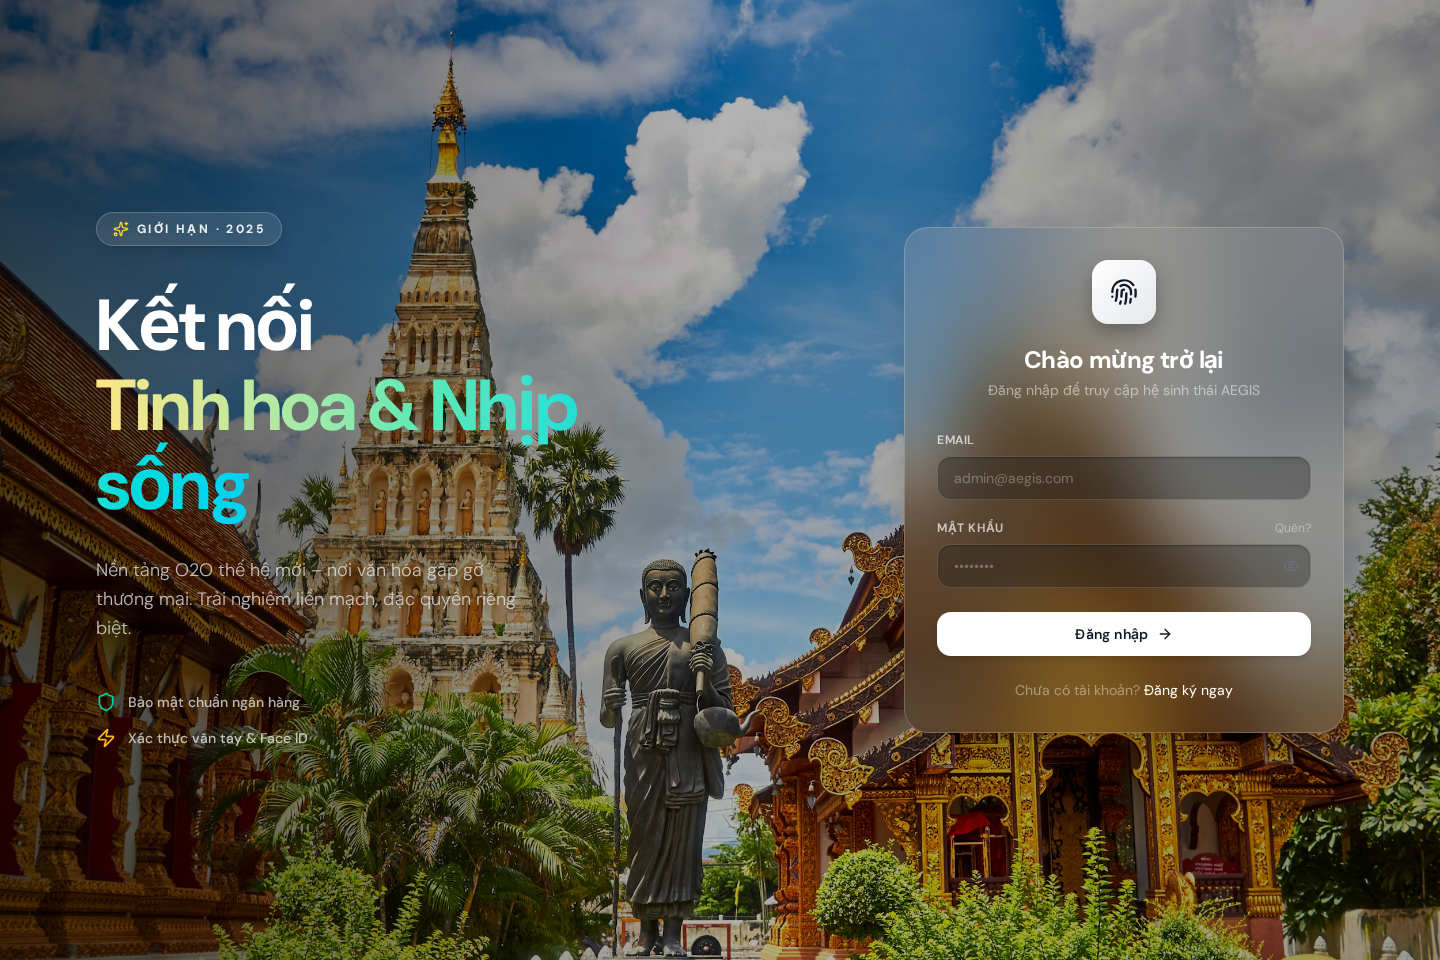
\includegraphics[width=\textwidth]{images/demo_login.png}
    \caption{Đăng nhập và khởi tạo phiên người dùng}
  \end{subfigure}
  \hfill
  \begin{subfigure}{0.49\textwidth}
    \centering
    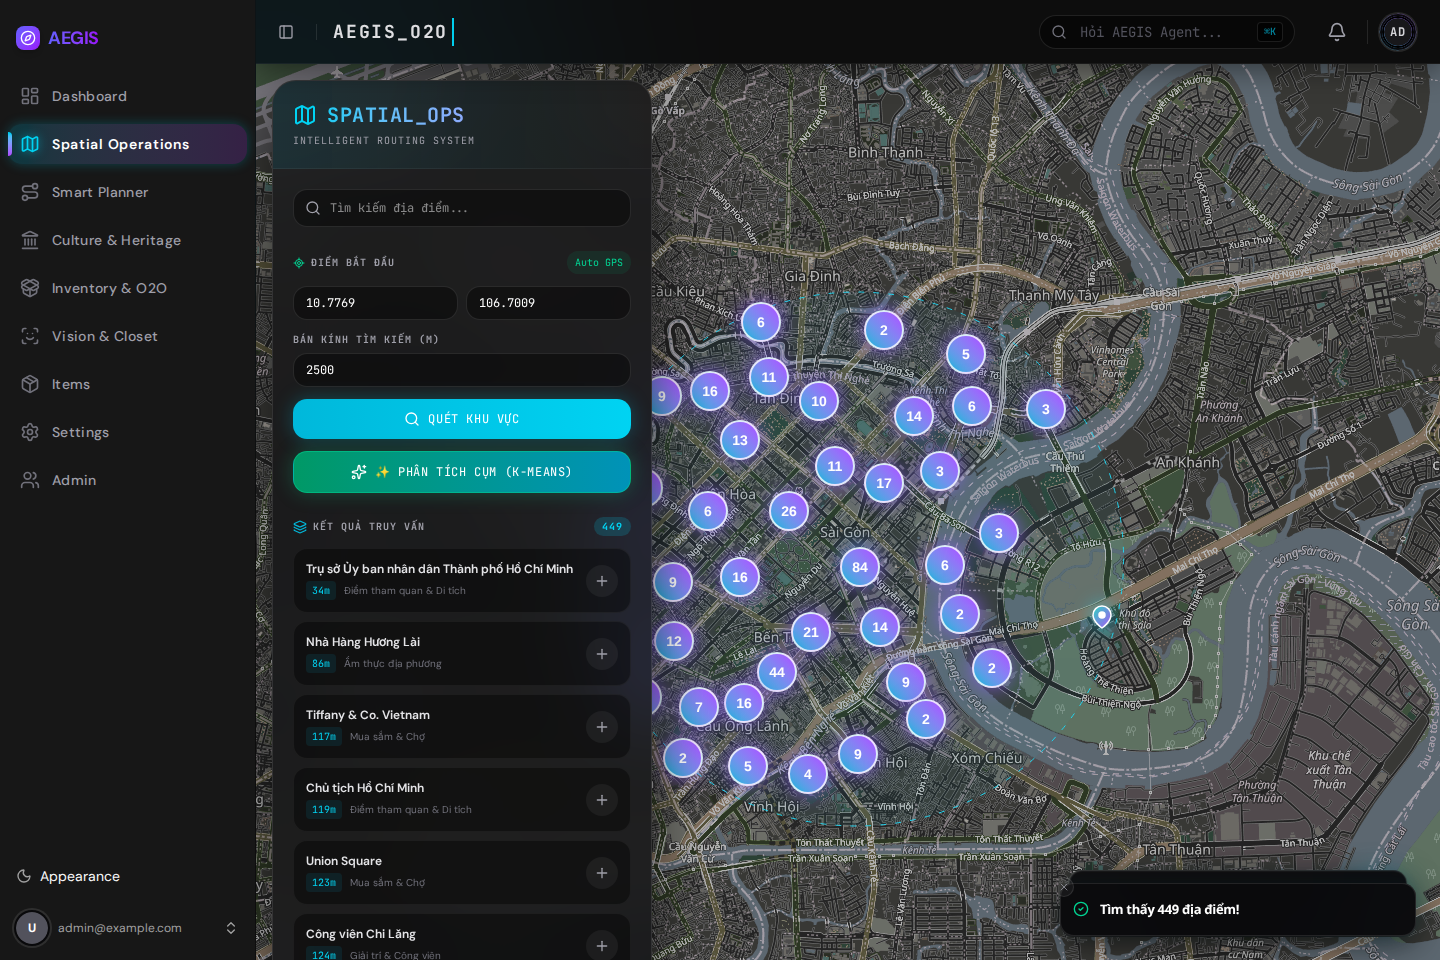
\includegraphics[width=\textwidth]{images/demo_spatial.png}
    \caption{Spatial Search quanh trung tâm TP.HCM}
  \end{subfigure}
  \caption{Kịch bản đăng nhập và khám phá địa điểm bằng bản đồ}
  \label{fig:demo_auth_spatial}
\end{figure}

\begin{figure}[H]
  \centering
  \begin{subfigure}{0.49\textwidth}
    \centering
    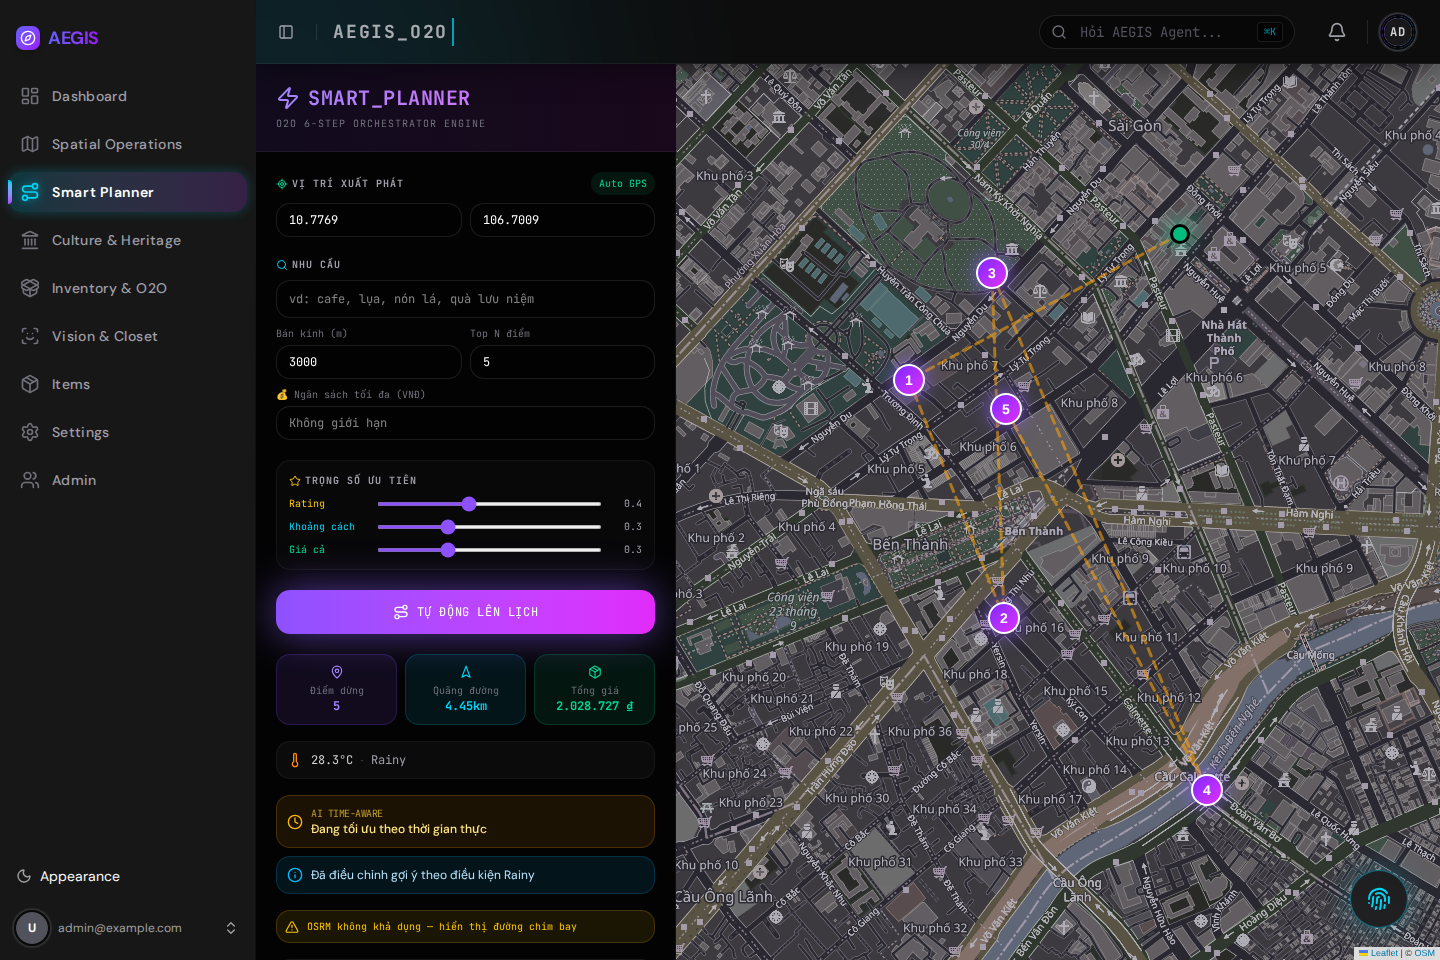
\includegraphics[width=\textwidth]{images/demo_itinerary.png}
    \caption{Smart Planner trả tuyến lộ trình tối ưu}
  \end{subfigure}
  \hfill
  \begin{subfigure}{0.49\textwidth}
    \centering
    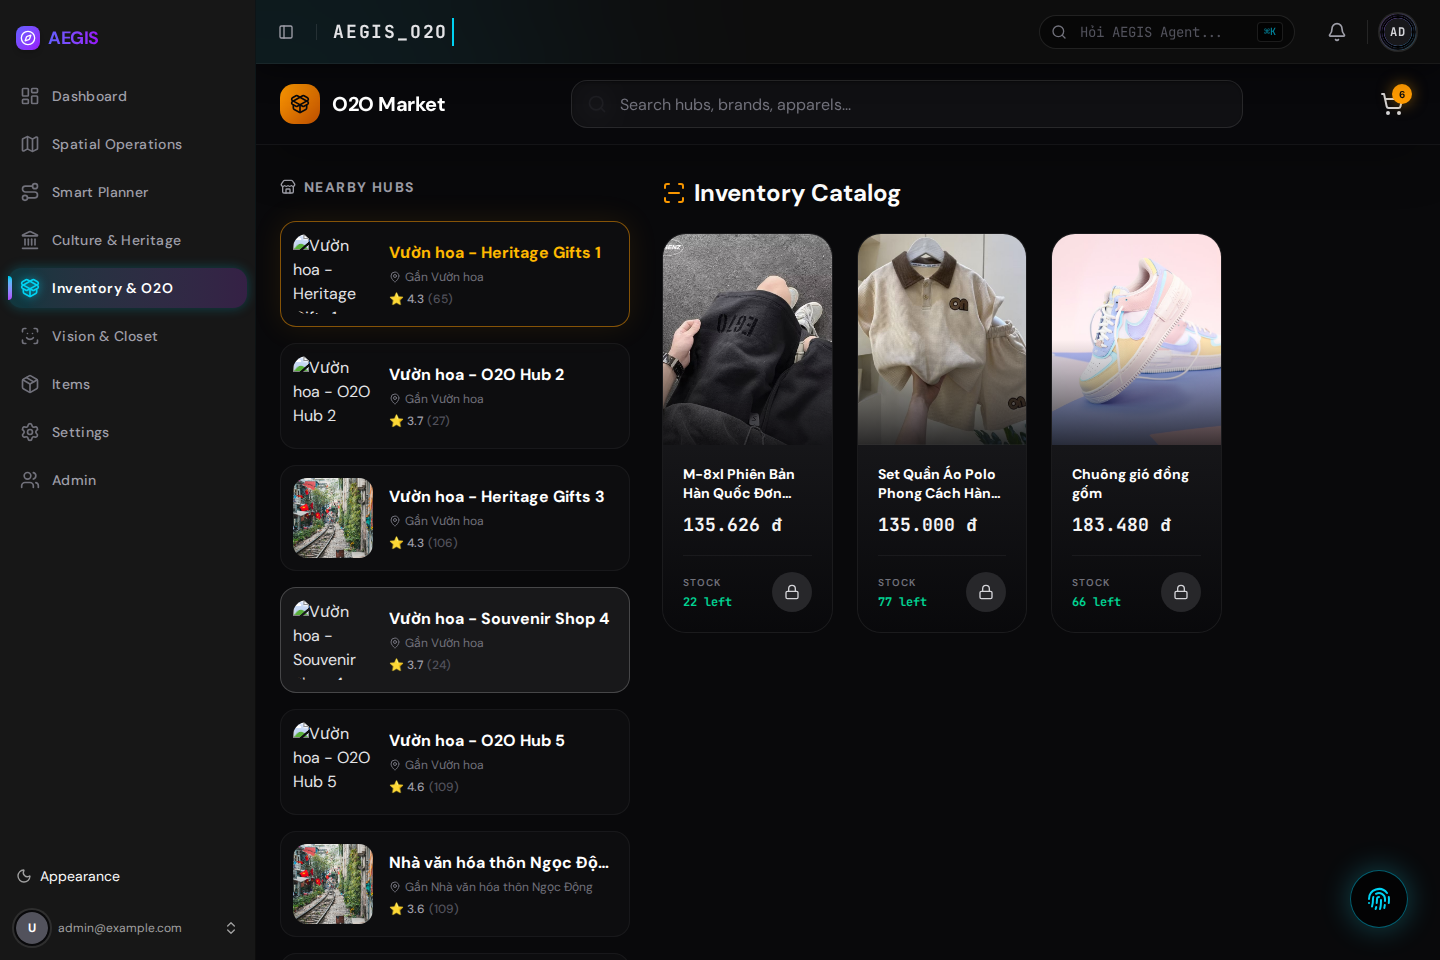
\includegraphics[width=\textwidth]{images/demo_inventory.png}
    \caption{Catalog O2O có ảnh, giá và tồn kho}
  \end{subfigure}
  \caption{Kịch bản lập lịch trình và xem catalog sản phẩm}
  \label{fig:demo_planner_inventory}
\end{figure}

\begin{figure}[H]
  \centering
  \begin{subfigure}{0.49\textwidth}
    \centering
    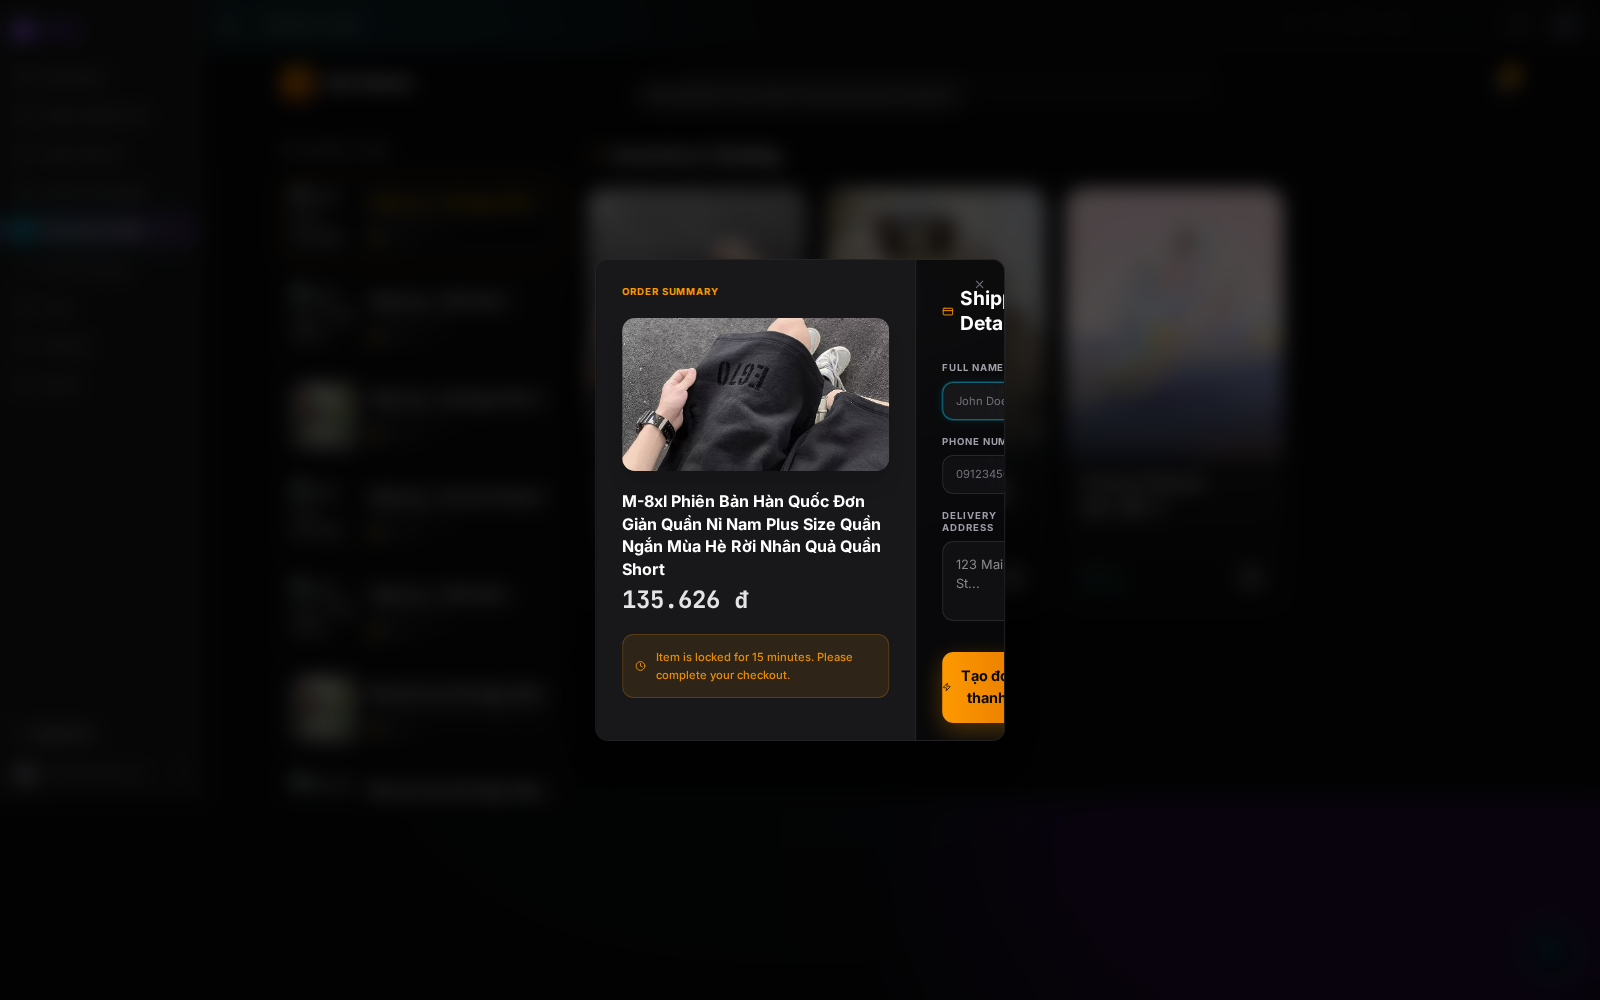
\includegraphics[width=\textwidth]{images/demo_o2o_lock.png}
    \caption{Giữ hàng O2O và chuyển sang checkout}
  \end{subfigure}
  \hfill
  \begin{subfigure}{0.49\textwidth}
    \centering
    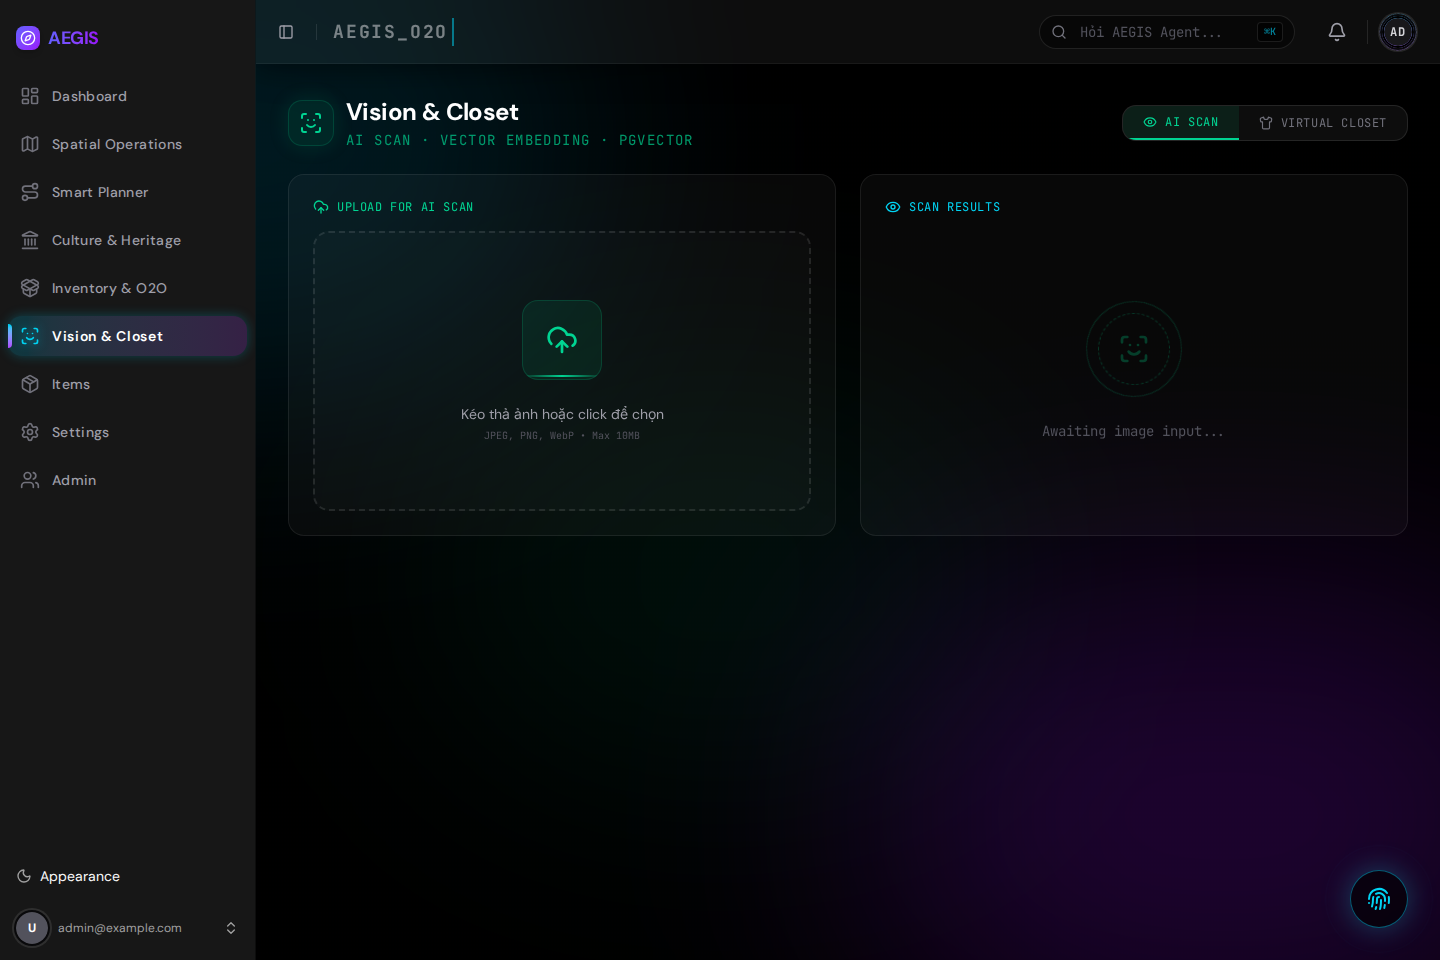
\includegraphics[width=\textwidth]{images/demo_vision.png}
    \caption{Visual Search/Vision Closet chờ ảnh upload}
  \end{subfigure}
  \caption{Kịch bản giao dịch O2O và tìm kiếm bằng ảnh}
  \label{fig:demo_o2o_vision}
\end{figure}

\begin{itemize}
    \item \textbf{Kịch bản đăng nhập:} người dùng đăng nhập bằng tài khoản quản trị mẫu. Sau khi xác thực thành công, frontend nhận phiên đăng nhập, gọi \texttt{/users/me} và mở các trang chức năng phía sau layout bảo vệ.

    \item \textbf{Kịch bản khám phá địa điểm:} người dùng nhập tọa độ \texttt{10.7769, 106.7009} và bán kính 2500m. Backend truy vấn PostGIS và trả 449 địa điểm quanh khu trung tâm TP.HCM; frontend hiển thị marker, danh sách kết quả và bán kính tìm kiếm trên bản đồ.

    \item \textbf{Kịch bản lập lịch trình thông minh:} người dùng chạy Smart Planner với bán kính 3000m, \texttt{top\_n=5} và bộ trọng số mặc định. Hệ thống lọc 29 ứng viên, chọn 5 điểm dừng, hiển thị tổng quãng đường 4.45km và tổng giá trị sản phẩm gợi ý khoảng 2,028,727.35đ. Trong phiên demo, OSRM không khả dụng nên giao diện hiển thị rõ trạng thái fallback đường chim bay; đây là hành vi mong đợi thay vì lỗi giao diện.
    
    \item \textbf{Kịch bản xem sản phẩm và giữ hàng:} người dùng mở trang Inventory/O2O, danh sách cửa hàng được lấy từ dữ liệu thật và catalog hiển thị sản phẩm có \texttt{image\_url}, giá, tồn kho còn lại. Khi bấm giữ hàng, hệ thống tạo lock 15 phút, mở checkout và yêu cầu người dùng hoàn tất thông tin nhận hàng trước khi tạo đơn thanh toán.

    \item \textbf{Kịch bản tìm kiếm bằng ảnh:} người dùng upload ảnh, frontend polling task cho đến khi worker hoàn tất. Chất lượng kết quả phụ thuộc lớn vào chất lượng \texttt{image\_url}, độ phủ embedding và khả năng mô hình hiểu đúng đặc trưng văn hóa địa phương. Vì vậy giao diện cần cho phép người dùng chuyển sang tìm kiếm văn bản hoặc lọc thủ công khi kết quả thị giác chưa phù hợp.
\end{itemize}

\clearpage
% ==============================================
% CHƯƠNG 7: KẾT LUẬN VÀ HƯỚNG PHÁT TRIỂN
% ==============================================
\section{Kết luận và hướng phát triển hệ thống}

\subsection{Kết quả trọng tâm đã đạt được}
Báo cáo đã trình bày quá trình phân tích và thiết kế nguyên mẫu AEGIS O2O dưới lăng kính của Tư duy tính toán.

\begin{enumerate}
    \item \textbf{Phương pháp luận thuật toán:} Vận dụng linh hoạt các thành tố cốt lõi bao gồm Phân rã, Nhận diện mẫu, Trừu tượng hóa và Thiết kế thuật toán nhằm xử lý có cấu trúc các bài toán trọng tâm của hệ thống (từ tối ưu hóa truy vấn không gian, định tuyến xấp xỉ TSP 2-Opt, kiểm soát tương tranh đến trích xuất đặc trưng hình ảnh bằng AI).
    
    \item \textbf{Kiến trúc hệ thống và kỹ nghệ phần mềm:} Thiết kế kiến trúc dịch vụ tách miền nghiệp vụ, trong đó các phân hệ API, cơ sở dữ liệu, bộ nhớ đệm, hàng đợi tác vụ và giao diện được đóng gói rõ ràng. Cách tổ chức này giúp hệ thống dễ kiểm thử, dễ thay thế từng thành phần và có nền tảng để mở rộng khi bổ sung hạ tầng quan sát, cân bằng tải và tự động phục hồi.
    
    \item \textbf{Giá trị ứng dụng thực tiễn:} Xây dựng được nguyên mẫu hỗ trợ du lịch thông minh, kết nối chu trình trải nghiệm của người dùng từ giai đoạn lập kế hoạch trực tuyến đến quá trình tương tác và giao dịch tại các cơ sở vật lý thực tế.
\end{enumerate}

\subsection{Những hạn chế tồn đọng}
Bên cạnh những kết quả đạt được, kiến trúc hệ thống hiện tại vẫn tồn tại một số điểm cần khắc phục:

\begin{itemize}
    \item \textbf{Tự động hóa đồng bộ trạng thái giao dịch:} Quy trình xác nhận hoàn tất luồng giao dịch O2O tại điểm bán vật lý hiện vẫn yêu cầu thao tác kiểm chứng thủ công từ phía nhân sự cơ sở kinh doanh, chưa được tự động hóa hoàn toàn vào luồng hệ thống lõi.
    
    \item \textbf{Ràng buộc về lưu trữ trạng thái cục bộ:} Phân hệ xử lý trực quan hiện đang lưu trữ dữ liệu tệp tin trực tiếp trên phân vùng vật lý cục bộ của máy chủ. Kiến trúc lưu trữ trạng thái này tạo ra rào cản kỹ thuật khi hệ thống có nhu cầu mở rộng quy mô ngang tự động trên môi trường phân tán.

    \item \textbf{Dữ liệu thực nghiệm còn hạn chế:} Dữ liệu địa điểm, cửa hàng và sản phẩm chủ yếu phục vụ minh họa chức năng. Script \texttt{fix\_product\_images.py} đang gán ảnh theo danh mục cửa hàng bằng keyword mapping và chọn ngẫu nhiên trong nhóm ảnh mẫu, nên ảnh có thể đúng ngữ cảnh nhưng chưa chắc đúng từng SKU. Khi triển khai thực tế, hệ thống cần bộ dữ liệu lớn hơn, có cập nhật định kỳ, kiểm tra trùng lặp và cơ chế xác minh chất lượng thông tin từ cửa hàng.

    \item \textbf{Chất lượng AI phụ thuộc ngữ cảnh:} Mô hình CLIP và LLM được sử dụng như thành phần hỗ trợ, không bảo đảm kết quả đúng tuyệt đối. Visual Search có thể nhầm lẫn với ảnh nhiễu, ảnh thiếu sáng, URL ảnh sản phẩm không đại diện đúng mặt hàng hoặc sản phẩm chưa có embedding; AI Agent có thể chọn sai công cụ nếu câu hỏi mơ hồ. Vì vậy hệ thống cần cơ chế xác thực tham số, fallback và phản hồi minh bạch cho người dùng.

    \item \textbf{Thiếu lớp quan sát vận hành đầy đủ:} Phiên bản hiện tại chưa trình bày sâu về logging tập trung, tracing phân tán, dashboard giám sát, cảnh báo khi worker chết hoặc khi tỉ lệ lock hết hạn tăng bất thường. Đây là điểm quan trọng nếu đưa hệ thống ra môi trường production.

    \item \textbf{Chưa hoàn thiện bài toán pháp lý và thanh toán thật:} Luồng VietQR/đặt giữ trong báo cáo mới dừng ở mức mô phỏng nghiệp vụ. Triển khai thương mại thật cần tích hợp cổng thanh toán, đối soát giao dịch, hoàn tiền, điều khoản bảo vệ người mua và quy trình xử lý tranh chấp với cửa hàng.
\end{itemize}

\subsection{Lộ trình phát triển mở rộng}
\begin{enumerate}
    \item \textbf{Lưu trữ đối tượng và ảnh sản phẩm thật:} Chuyển ảnh upload khỏi ổ đĩa cục bộ sang S3-compatible storage, đồng thời thay dần URL ảnh minh họa bằng ảnh sản phẩm thật do cửa hàng cung cấp để backend/worker có thể mở rộng ngang và kết quả tìm kiếm chính xác hơn.

    \item \textbf{Mở rộng dữ liệu O2O:} Bổ sung \texttt{opening\_hours}, \texttt{service\_radius}, trạng thái hoạt động của cửa hàng, bảng \texttt{product\_categories}, \texttt{embedding\_status} và quyền \texttt{is\_merchant} để tách rõ vai trò người bán khi hệ thống tiến tới vận hành thật.
    
    \item \textbf{Gợi ý cá nhân hóa:} Bổ sung lịch sử tìm kiếm, clickstream và đánh giá người dùng để xếp hạng địa điểm/sản phẩm sát nhu cầu hơn.
    
    \item \textbf{Ứng dụng di động:} Tận dụng GPS, camera và push notification để hỗ trợ tìm kiếm bằng ảnh và nhắc điểm đến/cửa hàng gần vị trí hiện tại.

    \item \textbf{Quan sát vận hành:} Tích hợp log tập trung, tracing và dashboard đo p95/p99 latency, task AI chờ xử lý, tỉ lệ lock hết hạn và tỉ lệ lỗi OSRM.

    \item \textbf{Bảo mật sản xuất:} Bổ sung secret manager, rotation khóa JWT, CSRF protection, kiểm tra file upload và audit log cho thao tác nhạy cảm.
\end{enumerate}

\clearpage
\section*{TÀI LIỆU THAM KHẢO}
\addcontentsline{toc}{section}{TÀI LIỆU THAM KHẢO}
\begin{enumerate}
\renewcommand{\labelenumi}{[\arabic{enumi}]}
    \item \textbf{PostGIS Project}. \textit{PostGIS 3.6 Official Manual}. Tài liệu hiện hành về kiểu dữ liệu không gian, chỉ mục GiST và các hàm \texttt{ST\_DWithin}, \texttt{ST\_Distance}. \url{https://postgis.net/documentation/manual/}.
    \item \textbf{PostgreSQL Global Development Group}. \textit{PostgreSQL Current Documentation: Explicit Locking}. Tài liệu hiện hành về khóa dòng, giao dịch và \texttt{SELECT FOR UPDATE}. \url{https://www.postgresql.org/docs/current/explicit-locking.html}.
    \item \textbf{Andrew Kane \& Contributors}. \textit{pgvector README}. Tài liệu cập nhật của phần mở rộng vector cho PostgreSQL, bao gồm Cosine distance, HNSW và cấu hình truy vấn ANN. \url{https://github.com/pgvector/pgvector}.
    \item \textbf{Celery Development Team}. \textit{Celery 5.6 Documentation}. Tài liệu stable hiện hành về distributed task queue, cơ chế acknowledge và retry. \url{https://docs.celeryq.dev/en/stable/}.
    \item \textbf{Project OSRM}. \textit{OSRM API Documentation v26.4.0}. Tài liệu hiện hành về Route, Table và Trip service phục vụ ma trận khoảng cách và lộ trình. \url{https://project-osrm.org/docs/v26.4.0/}.
    \item \textbf{FastAPI}. \textit{FastAPI Official Documentation}. Tài liệu hiện hành về xây dựng API Python, validation dữ liệu và OpenAPI docs. \url{https://fastapi.tiangolo.com/}.
    \item \textbf{OpenAI}. \textit{Function Calling / Tool Calling Documentation}. Tài liệu hiện hành về cách ràng buộc mô hình ngôn ngữ với công cụ và JSON schema. \url{https://platform.openai.com/docs/guides/function-calling}.
    \item \textbf{Redis}. \textit{SET command}. Tài liệu hiện hành về lệnh SET, tùy chọn hết hạn \texttt{EX/PX} và cách ghi khóa tạm có TTL. \url{https://redis.io/docs/latest/commands/set/}.
\end{enumerate}

\end{document}
bui